\documentclass{book}
\usepackage[a4paper,top=2.5cm,bottom=2.5cm,left=2.5cm,right=2.5cm]{geometry}
\usepackage{makeidx}
\usepackage{natbib}
\usepackage{graphicx}
\usepackage{stmaryrd}
\usepackage{multicol}
\usepackage{float}
\usepackage{listings}
\usepackage{color}
\usepackage{ifthen}
\usepackage[table]{xcolor}
\usepackage{textcomp}
\usepackage{alltt}
\usepackage{ifpdf}
\ifpdf
\usepackage[pdftex,
            pagebackref=true,
            colorlinks=true,
            linkcolor=blue,
            unicode
           ]{hyperref}
\else
\usepackage[ps2pdf,
            pagebackref=true,
            colorlinks=true,
            linkcolor=blue,
            unicode
           ]{hyperref}
\usepackage{pspicture}
\fi
\usepackage[utf8]{inputenc}
\usepackage{mathptmx}
\usepackage[scaled=.90]{helvet}
\usepackage{courier}
\usepackage{sectsty}
\usepackage{amsmath,amssymb}
\usepackage[titles]{tocloft}
\usepackage{doxygen}
\usepackage{command} % our own commands.
\lstset{language=C++,inputencoding=utf8,basicstyle=\footnotesize,breaklines=true,breakatwhitespace=true,tabsize=8,numbers=left }
\usepackage{amsfonts}
\makeindex
\setcounter{tocdepth}{2}
\renewcommand{\footrulewidth}{0.4pt}
\renewcommand{\familydefault}{\sfdefault}
\hfuzz=15pt
\setlength{\emergencystretch}{15pt}
\hbadness=750
\tolerance=750
\begin{document}
\hypersetup{pageanchor=false,citecolor=blue}
\begin{titlepage}
\vspace*{7cm}
\begin{center}
{\Large Documentation for Verdandi 1.5}\\
\vspace*{1cm}
{\large D. Chapelle, K. Charpentier, M. Fragu, V. Mallet, P. Moireau, C. Mouton}\\
\end{center}
\end{titlepage}
\clearemptydoublepage
\pagenumbering{roman}
\tableofcontents
\clearemptydoublepage
\pagenumbering{arabic}
\hypersetup{pageanchor=true,citecolor=blue}
\part{Introduction to Data Assimilation and Verdandi}
\chapter{Data Assimilation Principles}
\section{Motivations and basic definitions}

In order to obtain some information --~as detailed as possible --~on a \emph{natural system}, such as in geophysics, or regarding the important subcategory of \emph{living systems} which constitute the objects of study in biology and medicine, the most straightforward strategy consists in obtaining \emph{measurements} on the system at hand. Note that we deliberately use the term measurement, related but not reduced to \emph{experiments}, to signify that it is not in general possible to design specific experiments allowing to determine all kinds of physical properties of the system --~as is done for instance for industrial systems. By contrast, natural systems induce drastic limitations in measurements, in that they generally must be ``taken as they are'', namely, observed in their current operating conditions, whether this is due to the practical impossibility of apprehending them comprehensively (e.g.~in geophysics), or to the undesirable character of any strong perturbation of the system (invasiveness in living systems).

Specializing now our discussion on living systems, abundant measurements are frequently at hand, in the form of clinical images and signals of various origins. Despite the diversity and rich information contents of these data, they are also inevitably limited in many respects. Beside considerations on sampling and noise, this holds in particular as regards:
\begin{itemize}
	\item their extent: for example only 2D measurements, or boundary information, may be available for a 3D system, or only part of the whole domain;
	\item their type: some quantities are never measured, such as internal stresses in a living tissue, or various physical constitutive parameters (stiffness, contractility, etc.).
\end{itemize}

Nevertheless, we may want to consider \emph{physical models} to describe and predict the behavior of these systems. Clearly, these models may be seen as providing some complementary information on the system. However, their predictivity requires the careful adjustment of many parameters --~in particular regarding the detailed geometry (anatomy), physical properties, boundary conditions and initial conditions needed in the model --~most of which being out of reach of the available measurements.

The purpose of \emph{data assimilation} is then to combine the information available from these two sources --~measurements on the one hand, and models and the other hand --~by seeking an adequate compromise between:
\begin{itemize}
	\item the discrepancy computed between simulations of the model and the corresponding measurements;
	\item the \emph{a priori} confidence in the model, since errors are also present in the measurements.
\end{itemize}
The desired output of this procedure is an estimation of the unknown quantities of interest, namely,
\begin{itemize}
	\item state variables (the ``trajectories'' of the system), and in particular their initial values at a given reference time;
	\item physical parameters which must be prescribed in the model equations.
\end{itemize}
In terms of clinical applications, the expected benefits are to assist and improve both \emph{diagnosis} and \emph{prognosis}:
\begin{itemize}
	\item diagnosis, by providing more complete information on the patient (spatially-distributed quantities, and various otherwise unreachable indicators), and with improved accuracy;
	\item prognosis, since once data assimilation has been performed the model can be more confidently used to predict natural or artificial evolutions of the system, for example to simulate the effect of various possible therapeutic strategies.
\end{itemize}

We will now introduce some basic notation necessary to discuss the fundamental principles of data assimilation. First of all, we consider physical models in the form of dynamical systems governed by equations of the type
\begin{equation}\label{eq:modelNotation}
	\dot{x} = \mathcal{M}(x,p,t).
\end{equation}
In this equation, $x$ denotes the so-called \emph{state variable}, namely, the physical quantity which the model aims at describing in its time-wise evolution --~hence, the time derivative in the left-hand side --~and also frequently spatial variations for distributed quantities. In this generic notation, the whole model is essentially summarized in the so-called \emph{dynamical operator} $\mathcal{M}$, which applies on the state variable itself, and may depend on time $t$ as well as on a set of physical parameters denoted by $p$. This operator may arise from various types of physical formulations, e.g.~in solid and fluid mechanics or electrophysiology. Mathematically speaking, it may take the form of partial differential equations (PDEs) or ordinary differential equations (ODEs, namely, only differentiated with respect to the time variable), or algebraic systems, in particular.

Clearly, in such model formulations we need to prescribe --~hence to estimate when unknown via the data assimilation procedure --~the initial condition $\mathcal{M}(0)$ and the parameter vector $p$. Typically, in the models considered the state variable may contain a large number of scalar coefficients --~typically $10^3$ to $10^7$ degrees of freedom in a continuum mechanics model --~whereas the size of the parameter vector is generally much more limited, and in practice we seldom have to estimate more than a few hundreds of parameter values. Once the initial condition and the parameter vector associated with \eqref{eq:modelNotation} are estimated, the model can be simulated in time, using appropriate numerical techniques.

Another important notation concerns the measurements, typically represented by an equation of the type
\begin{equation}\label{eq:measNotation}
	y = \mathcal{H}(x,t) + e^o,
\end{equation}
where $y$ denotes the actual data, $\mathcal{H}$ is the so-called \emph{observation operator}, and $e^o$ accounts for the error inherent to the measurement process, often called the \emph{noise}. Note that the quantity $y$ will frequently correspond to pre-processed --~not raw --~data, for example images processed with segmentation or optical flow techniques in order to extract some position, displacement or velocity information. We further emphasize that this equation also represents a model --~in this case of the measurements --~where modeling ingredients are embedded both in the expression of $\mathcal{H}$ and the characterization of $e^o$, which may be of probabilistic or deterministic nature.


\section{Fundamental principles}

We are now in a position to introduce some fundamental principles for data assimilation procedures. First of all, there are two main categories of methods: variational and sequential methods.

\subsection{Variational procedures}

In variational procedures, we consider a criterion to be minimized in order to achieve the above-mentioned compromise between simulation-measurements discrepancy and model confidence, see e.g.~\cite{Bensoussan71,Chavent10} and references therein. A typical criterion would read
\begin{equation}\label{eq:varCriterion}
	\mathcal{J}_T(\varstate_\state,\varstate_{\param}) = \int_0^T \|\observ-\obsOp(\state)\|_{\obsNoiseNorm}^2 \, dt + \|\varstate_\state\|_{(\initNoiseCov)^{-1}}^2 + \|\varstate_{\param}\|_{(\paramNoiseCov)^{-1}}^2,
\end{equation}
where $\|.\|_{\obsNoiseNorm}$, $\|.\|_{(\initNoiseCov)^{-1}}$ and $\|.\|_{(\paramNoiseCov)^{-1}}$ denote suitable norms for each quantity concerned, and associated with the matrices appearing as subscripts. In this criterion, $\state$ is constrained to satisfy the model equation \eqref{eq:modelNotation} starting from the initial condition $\state(0)=\state_0+\initNoise_\state$ and with parameter values given by $\param=\param_0+\initNoise_\param$. In order to perform this minimization, a classical strategy consists in computing the gradient of the criterion, which requires the simulation of the so-called \emph{adjoint model}. The adjoint model equation is an evolution system closely related to --~and inferred from, indeed --~the direct model equation \eqref{eq:modelNotation}, viz.
\begin{equation}\label{eq:adjointPb}
	\begin{cases}
	\dot{\adjoint}_\state + \frac{\partial \modelOp}{\partial \state}^\intercal \adjoint_\state = -\frac{\partial \obsOp}{\partial \state}^\intercal\obsNoiseNorm(\observ-\obsOp(\state)) \\
	\adjoint_\state(T) = 0 \\
	\dot{\adjoint}_{\param} + \frac{\partial \modelOp}{\partial \param}^\intercal\adjoint_\state= 0 \\
	\adjoint_{\param}(T) = 0
	\end{cases}
\end{equation}
These equations must be simulated backwards in time from the final time $T$ to the initial time in order to obtain the gradient value criterion expressed as
\[
	\begin{cases}
		\diff_{\varstate_\state}\mathcal{J} \cdot \delta \varstate_\state = {\varstate_\state}^\intercal (\initNoiseCov)^{-1} \delta \varstate_\state - \adjoint_\state(0)^\intercal \delta \varstate_\state\\
		\diff_{\varstate_{\param}}\mathcal{J} \cdot \delta \param = {\varstate_\param}^\intercal (\paramNoiseCov)^{-1} \delta \varstate_\param - \adjoint_{\param}(0)^\intercal \delta \varstate_\param,
	\end{cases}
\]
Hence, each gradient computation requires the forward simulation of the direct model and the backward simulation of the adjoint, and this must be repeated until convergence of the minimization algorithm. Figure \ref{fig:variat} illustrates this iterative procedure, and the fact that observability can be improved by considering a longer time window, hence, also more measurements. This type of variational procedure is also referred to as ``4DVar'' in the data assimilation community, while ``3DVar'' is used to refer to minimization estimation performed for static models, or for dynamic models at a given time (namely, without time integral).

\begin{figure}[htbp]
\begin{center}
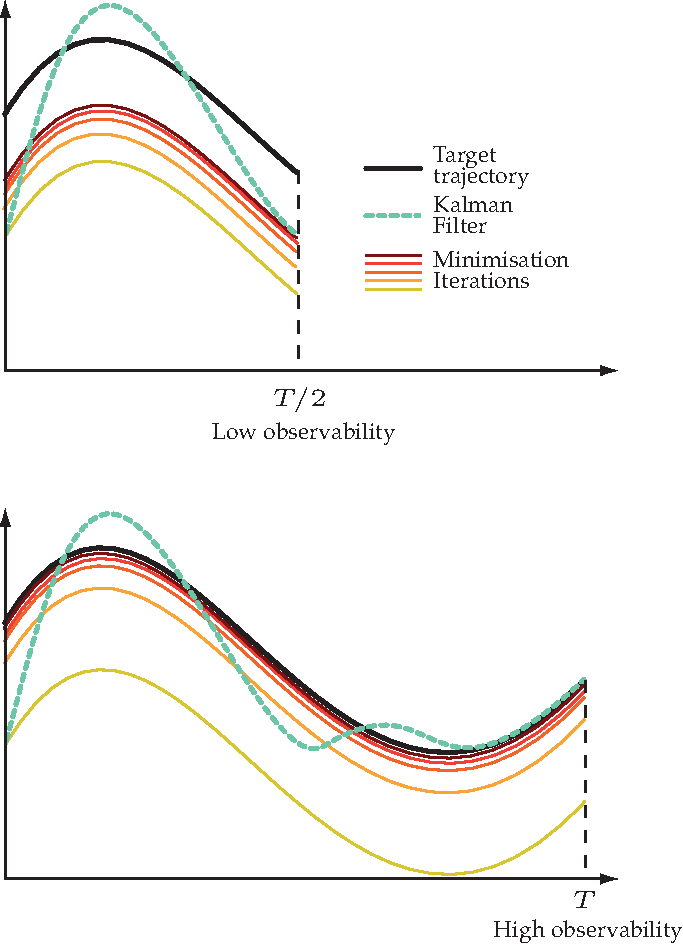
\includegraphics[width=.5\textwidth]{figure/seqVSvaria.pdf}
\caption{Schematic of minimization iterations and Kalman filter tracking on a sliding time window (as seen via one single output)}
\label{fig:variat}
\end{center}
\end{figure}

Concerning the time discretization, it is classical to formulate an optimal discrete time minimization criterion and find its corresponding adjoint rather than discretizing directly \eqref{eq:adjointPb}. Hence, we consider a criterion of the form
\begin{equation}\label{eq:varCriterionTimeDisc}
	J_N(\varstate_\state,\varstate_{\param}) = \sum_{k=0}^N \|\observDof_k-\obsOpDof(\stateDof_k)\|_{\obsNoiseNormDof_k}^2 \,  + \|\varstateDof_\state\|_{(\initNoiseCovDof)^{-1}}^2 + \|\varstateDof_{\param}\|_{(\paramNoiseCovDof)^{-1}}^2,
\end{equation}
with for example $\obsNoiseNormDof_k = \Delta t \obsNoiseNormDof$.

\subsection{Sequential procedures}

By contrast, sequential procedures --~also often referred to as \emph{filtering} --~proceed by simulating equations closely resembling the direct model equations, with an additional correction term taking into account the discrepancy between the simulation and the actual measurements, namely $y-\mathcal{H}(x)$, quantity called the \emph{innovation}. For example when only the initial condition is unknown the filtering equation would be of the type
\begin{equation}\label{eq:filterNotation}
	\dot{\state^a} = \modelOp(\state^a,t) + K(\observ-\obsOp(\state^a)),
\end{equation}
where the operator $K$ --~frequently linear --~is called the \emph{filter}. The filtering equation simulation is then started from the candidate initial condition $X_0$, and the aim of the correction is to bring the simulated trajectory close to the target system, see Fig.~\ref{fig:variat}.

This type of strategy was made extremely popular by the Kalman theory, which formulated an optimal setting for deriving the filter operator, initially when the operators $A$ and $H$ are both linear. In this case, the Kalman equations read
\begin{equation}\label{eq:Kalman}
	\begin{cases}
		\dot{\state^a} = \modelOp\state^a + \Cov\obsOp^\intercal \obsNoiseNorm (\observ-\obsOp\state^a)\\
		\dot{\Cov} - \Cov\modelOp^\intercal - \modelOp\Cov + \Cov\obsOp^\intercal \obsNoiseNorm \obsOp\Cov = 0\\
		\Cov(0)=\initNoiseCov\\
		\state^a(0) = \stateAug_\diamond
	\end{cases}
\end{equation}
where $W$ and $P_0$ denote the  so-called covariance matrices of the measurement noise and initial condition uncertainty, respectively. We can see that the filter expression is based on the computation of the time-dependent covariance matrix $P$ which satisfies a Riccatti equation. In fact, in the linear case the variational and Kalman procedures can be shown to be exactly equivalent, and the minimizing direct and adjoint states ($X_\text{inf}$ and $p_\text{inf}$, respectively) are related to the Kalman filter by the identity \cite{Bensoussan71}
\[
	\stateAug_\infty = \state^a + \Cov \adjoint_\infty.
\]
This is also illustrated in Figure \ref{fig:variat} where we show that the Kalman estimation coincides with the minimizing solution at the end of the time window considered.

When nonlinearities are to be considered, various extensions are available, and in particular the Extended Kalman Filtering (EKF) approach, in which the linearized forms of the operators are used in the filter equation. However, in such a case the approach is no longer equivalent to the variational setting. Nevertheless, some alternative filter equations can be derived from the variational formulation, but the filter computation then requires solving a Hamilton-Jacobi-Bellman equation in a space which has the dimension of the state variable \cite{Moireau08}, which is in general not practical.

Note that, in practice, the Kalman (or EKF) approach itself is also quite limited as regards the size of the system which can be handled, since the covariance matrix $\Cov$ has the size of the state variable, and is a dense matrix, unlike the dynamical operators. In order to circumvent this limitation some alternative approaches must be considered.

Concerning time discretization, it is classical to formulate the optimal filter directly from the optimal time-discrete minimization criteria rather than discretizing directly \eqref{eq:Kalman}. Hence, after some quite tedious computations, we can formulate a prediction-correction scheme
\begin{subequations}\label{eq:KalmanDiscrete}
	\begin{enumerate}
	\item Prediction:
   \begin{align}
   	\begin{cases}
   		\hat{\stateDof}_{h+1}^f &= \modelOp_{h}(\stateDof_h^a) \\
   		\CovDof_{h+1}^f &= \frac{\partial \modelOpDof_{h}}{\partial \stateDof} \CovDof_{h}^a \frac{\partial \modelOpDof_{h}}{\partial \stateDof}^\intercal
   	\end{cases}
   \end{align}
	\item Correction:
   \begin{align}\label{eq:KalmanCorrection}
   	\begin{cases}
   		\CovDof_{h+1}^a &= \left(\frac{\partial \obsOpDof_{h+1}}{\partial \stateDof} ^\intercal\obsNoiseCovDof_{h+1}^{-1} \frac{\partial \obsOpDof_{h+1}}{\partial \stateDof} + (\CovDof_{h+1}^f)^{-1}\right)^{-1} \\
		\gainOpDof_{h+1} &= \CovDof_{h+1}^a \frac{\partial \obsOpDof_{h+1}}{\partial \stateDof}^\intercal \obsNoiseCovDof_{h+1}^{-1} \\
		\hat{\stateDof}_{h+1}^a  &= \hat{\stateDof}_{h+1}^f + \gainOpDof_{h+1}(\observDof_{h+1}- \obsOpDof_{h+1}(\hat{\stateDof}_{h+1}^f))
   	\end{cases}
   \end{align}
\end{enumerate}
\end{subequations}


For the sake of simplicity, we have introduced the Kalman filter in a deterministic context, but the probabilistic counterpart exists. In a linear framework the expressions are exactly the same, albeit with the additional interpretation
\begin{equation}\label{eq:proba}
	\begin{cases}
			\text{a priori mean: } \hat{\stateDof}_{h+1}^f = \E(\stateDof_{h+1}|\observDof_0,\ldots,\observDof_h),	\\
			\text{a priori covariance: }  \CovDof_{h+1}^f = \E\bigl((\stateDof_{h+1}-\hat{\stateDof}_{h+1}^f)(\stateDof_{h+1}-\hat{\stateDof}_{h+1}^f)^\intercal\bigr), \\
			\text{a posteriori mean: } \hat{\stateDof}_{h+1}^a = \E\bigl(\stateDof_{h+1}|\observDof_0,\ldots,\observDof_{h+1}\bigr), \\
			\text{a posteriori covariance: } \CovDof_{h+1}^a = \E((\stateDof_{h+1}-\hat{\stateDof}_{h+1}^a)(\stateDof_{h+1}-\hat{\stateDof}_{h+1}^a)^\intercal),
	\end{cases}
\end{equation}

This results extend to the non-linear context with the EKF \eqref{eq:KalmanDiscrete} but the identities \eqref{eq:proba} are then only approximate. To improve the quality of this approximation, the Unscented Kalman Filter has then been introduced \cite{Julier00}, based on the idea of substituting means and covariances by empirical quantities computed from sample points:
\begin{equation}\label{eq:probaEmpirical}
	\begin{cases}
			\hat{\stateDof}_{h+1}^f = \sum_{i=1}^d \alpha_i\stateDof_{h+1}^{[i]-},	\\
			\CovDof_{h+1}^f = \sum_{i=1}^d \alpha_i(\stateDof_{h+1}^{[i]-}-\hat{\stateDof}_{h+1}^f)(\stateDof_{h+1}^{[i]-}-\hat{\stateDof}_{h+1}^f)^\intercal, \\
			\hat{\stateDof}_{h+1}^a = \sum_{i=1}^d \alpha_i\stateDof_{h+1}^{[i]+}, \\
			\CovDof_{h+1}^a = \sum_{i=1}^d \alpha_i(\stateDof_{h+1}^{[i]+}-\hat{\stateDof}_{h+1}^a)(\stateDof_{h+1}^{[i]+}-\hat{\stateDof}_{h+1}^a)^\intercal,
	\end{cases}
\end{equation}
with $\sum_{i=1}^d \alpha_i = 1$.

In practice, the correction particles are sampled around the mean $\hat{\stateDof}_{h}^a$ with a covariance $\CovDof_{h}^a$ and the prediction samples then verify
\begin{subequations}\label{eq:UKFDiscrete}
\begin{equation}
	\stateDof_{h+1}^{[i]-} = \modelOpDof(\stateDof_{h}^{[i]+}).
\end{equation}
Then, by computing
\begin{equation}
	\observDof_{h+1}^{[i]-} = \obsOpDof(\stateDof_{h+1}^{[i]-}),\quad  \observDof_{h+1}^{-} = \sum_{i=1}^d \alpha_i \observDof_{h+1}^{[i]}
\end{equation}
The gain is defined by
\begin{equation}
\begin{cases}
		\gainOpDof_{h+1} = (\CovDof_{h+1}^{\stateDof,\observDof}) \cdot (\CovDof_{h+1}^{\observDof,\observDof})^{-1} \\
		\CovDof_{h+1}^{\stateDof,\observDof} = \sum_{i=1}^d \alpha_i(\stateDof_{h+1}^{[i]-}-\hat{\stateDof}_{h+1}^f)(\observDof_{h+1}^{[i]-}-\observDof_{h+1}^{-})^\intercal\\
		\CovDof_{h+1}^{\observDof,\observDof} = \sum_{i=1}^d \alpha_i(\observDof_{h+1}^{[i]-}-\observDof_{h+1}^{-})(\observDof_{h+1}^{[i]-}-\observDof_{h+1}^{-})^\intercal + W_{h+1}
\end{cases}
\end{equation}
so that we keep having
\begin{equation}
\begin{cases}
	\hat{\stateDof}_{h+1}^a  = \hat{\stateDof}_{h+1}^f + \gainOpDof_{h+1}(\observDof_{h+1}- \observDof_{h+1}^{-}) \\
	\CovDof_{h+1}^a = \CovDof_{h+1}^f - \CovDof_{h+1}^{\stateDof,\observDof}  (\CovDof_{h+1}^{\observDof,\observDof})^{-1} 	(\CovDof_{h+1}^{\stateDof,\observDof})^\intercal
\end{cases}
\end{equation}
\end{subequations}
and proceed recursively with new correction particles $\stateDof_{h+1}^{[i]+}$.


The Ensemble Kalman Filter, introduced in \cite{EVENSEN:1994tl}, follows the same principles of approximating the covariances by sampled particles with, most of the time, an increased number of particles with respect to the UKF filter, and various ways of sampling the particles around the mean value. Finally Monte Carlo strategies exploit  a very large number of particles to give a better approximation of the non-linear optimal filter but the practical details of these methods are beyond the scope of this review focused on large dimensional systems coming from the discretization of PDEs.


\subsection{Reduced-order sequential strategies}\label{sec:RO}

\paragraph{Reduced-Order Extended Kalman Filtering (ROEKF)}

In order to deal with the limitations of sequential strategies due to the system size, a classical strategy consists in assuming a specific reduced-order form for the covariance operators. For example, making the ansatz
\begin{equation}\label{eq:red-order-princ}
	\forall t,\quad \Cov(t) = L(t) U(t)^{-1} L(t)^\intercal
\end{equation}
with $U$ an invertible matrix of small size $r$ and $L$ an extension operator, we can show that within linear assumptions the solution of the Riccatti equation in \eqref{eq:Kalman} reduces to
\begin{equation}\label{eq:reducedDynamics}
	\dot{L} = \modelOp L \text{ and }
	\dot{U} = L^\intercal \obsOp^\intercal \obsNoiseNorm \obsOp L.
\end{equation}
which is actually computable in practice.

In a non-linear framework, we can then approximate the covariance dynamics by extending \eqref{eq:reducedDynamics} as
\begin{equation}\label{eq:nl-reducedDynamics}
	\dot{L} = \frac{\partial \modelOp}{\partial \stateAug} L \text{ and }
	\dot{U} = L^\intercal \frac{\partial \obsOp}{\partial \stateAug}^\intercal \obsNoiseNorm \frac{\partial \obsOp}{\partial \stateAug} L.
\end{equation}
These strategies have relevant applications in the case of parameter identification \emph{per se}. It is common, indeed, to assume more space regularity for the parameters than for the state initial condition. Hence, after discretization the parameters can be represented by a small number of degrees of freedom. Assuming that we can limit $U(0)$ to the parametric space, the extension operator can then be decomposed into two components $L = \left( \begin{smallmatrix} \LX \\ \Ltheta \end{smallmatrix} \right)$ with $\Ltheta = \1$ and
\begin{equation}\label{eq:sensitivity}
	\dot{L}_\state = \frac{\partial \modelOp}{\partial \state} \LX + \frac{\partial \modelOp}{\partial \param}.
\end{equation}
We recognize in this expression the dynamics of the sensitivity operator $\frac{\partial \state}{\partial \param}$, which provides a nice interpretation for this strategy of uncertainty covariance reduction. Furthermore, in the linear framework we can prove that this sequential estimator corresponds to the optimal filter associated with the criterion
\begin{equation}\label{eq:paramCriterion}
	\mathcal{J}(\varstate_{\param}) = \int_0^T \|\observ-\obsOp(\state)\|_{\obsNoiseNorm}^2 \, dt +  \|\varstate_{\param}\|_{(\paramNoiseCov)^{-1}}^2,
\end{equation}
where $\state$ follows the trajectory associated with $\varstate_{\param}$ and fixed initial condition, which is commonly used in variational identification procedures. All this justifies naming this strategy \emph{Reduced-Order Extended Kalman Filter} (ROEKF), but it is also known as \emph{Singular Evolutive Extended Kalman Filter} following the work of \cite{Pham:1998p44}.

This concept can be applied directly on time and space discretized versions of the equations, which leads to a \emph{discrete time Reduced-Order Extended Kalman Filter}.
\begin{subequations}\label{eq:ROKalmanDiscrete}
	\begin{enumerate}
	\item Prediction:
   \begin{align}
   	\begin{cases}
   		\hat{\stateDof}_{h+1}^f &= \modelOpDof_{h} (\stateDof_{h}^a) \\
   		L_{h+1} &= \frac{\partial \modelOpDof_{h}}{\partial \stateDof}  L_h
   	\end{cases}
   \end{align}
	\item Correction:
   \begin{align}
   	\begin{cases}
   		U_{h+1} &= U_{h} + L_{h+1}^\intercal \frac{\partial \obsOpDof_{h+1}}{\partial \stateDof}^\intercal \obsNoiseCovDof^{-1}_{h+1} \frac{\partial \obsOpDof_{h+1}}{\partial \stateDof} L_{h+1} \\
		\gainOpDof_{h+1} &= \CovDof_{h+1}^a \frac{\partial \obsOpDof_{h+1}}{\partial \stateDof}^\intercal\obsNoiseCovDof_{h+1}^{-1} \\
		\hat{\stateDof}_{h+1}^a  &= \hat{\stateDof}_{h+1}^f + \gainOpDof_{h+1}(\observDof_{h+1}- \obsOpDof_{h+1} \hat{\stateDof}_{h+1}^f)
   	\end{cases}
   \end{align}
\end{enumerate}
\end{subequations}

\paragraph{Reduced-Order Unscented Kalman Filtering (ROUKF)}

Alternatively, this strategy can be coupled with the UKF approach by showing that particles can be generated only in the space of small dimension and the computation made in the UKF filter \eqref{eq:UKFDiscrete} can be compatible with the time discretized counterpart of \eqref{eq:red-order-princ}. This was proven in \cite{PM-DC-10,moireau-chapelle-11err} which also provided a very general version of the \emph{Reduced Order Unscented Kalman Filter} (ROUKF). In particular this algorithm is close to the \emph{Singular Evolutive Interpolated Kalman Filter} \cite{pham01stochastic,hoteit-pham-blum-02} for a choice of particles $d = r+1$ and reads as follows.
\paragraph{Algorithm~--} Given an adequate sampling rule, we store the corresponding weights in the diagonal matrix $\mathbf{D}_\alpha$ and precompute so-called unitary sigma-points (i.e.~with zero mean and unit covariance) denoted by $(\vec{I}^{[i]})_{1\leq i \leq r+1}$; we then perform at each time step
\begin{subequations}
	\begin{enumerate}
		\item Sampling:
	\begin{align}
		\begin{cases}
			C_h &= \sqrt{(U_h)^{-1}} \\[0.1cm]
			\hat{\stateDof}^{[i]+}_{h} &= \hat{\stateDof}_{h}^a + L_h \cdot C_h^\intercal \cdot \vec{I}^{[i]},\quad 1\leq i \leq r+1 \\[0.1cm]
		\end{cases}
	\end{align}
	\item Prediction:
   \begin{align}
   	\begin{cases}
   		\hat{\stateDof}^{[i]-}_{h+1} &= \modelOpDof_{h}(\hat{\stateDof}^{[i]+}_{h}),\quad 1\leq i \leq r+1 \\[0.1cm]
   	   	\hat{\stateDof}^f_{h+1} &= \sum_{i=1}^{r+1} \alpha_i \hat{\stateDof}_{h+1}^{[i]-}\\[0.1cm]
   	\end{cases}
   \end{align}
	\item Correction:
   \begin{align}
   	\begin{cases}
   		L_{h+1} &= [\hat{\stateDof}^{[*]-}_{h+1}]\mathbf{D}_\alpha [\vec{I}^{[*]}]^\intercal \\[0.1cm]
   		\observDof_{h+1}^{[i]-} &= \obsOpDof_{h+1}(\hat{\stateDof}^{[i]-}_{h+1}) \\[0.1cm]
		\observDof_{h+1}^f &= \sum_{i=1}^{r+1} \alpha_i \observDof_{h+1}^{[i]-} \\[0.1cm]
   		\mathbf{\Gamma}_{h+1} &=  [\observDof^{[*]-}_{h+1}]\mathbf{D}_\alpha [\vec{I}^{[*]}]^\intercal \\[0.1cm]
   		U^{n+1} &=  \mathbf{1} + \mathbf{\Gamma}_{h+1}^\intercal  \obsNoiseCovDof_{h+1}^{-1} \mathbf{\Gamma}_{h+1} \\[0.1cm]
   		\hat{\stateDof}_{h+1}^a &= \hat{\stateDof}_{h+1}^f - L_{h+1} U^{n+1}  \mathbf{\Gamma}_{h+1}^\intercal \obsNoiseCovDof_{h+1}^{-1}  (\observDof_{h+1} - \observDof_{h+1}^f)
   	\end{cases}
   \end{align}
\end{enumerate}
\end{subequations}
where we denote by $[\vec{I}^{[*]}]$ the matrix concatenating the $(\vec{I}^{[i]})$ vectors side by side, and similarly for other vectors.


\subsection{Luenberger observers}

The so-called \emph{observer theory}, initiated by Luenberger \cite{Luenberger63}, is based on the simple realization that, defining the estimation error
\[
	\tilde{\state} = \state - \state^a,
\]
we obtain in the linear case, when subtracting the direct model and filtered equations, the dynamics
\begin{equation}
	\dot{\tilde{\state}} = (\modelOp-\gainFilter\obsOp) \tilde{\state} - \gainFilter\chi.
\end{equation}
This type of dynamical equation is well-known is control theory: it is similar to the closed-loop controlled equation of a system of natural dynamics governed by $\modelOp$, and submitted to a feedback control defined by the operator $\gainFilter$ applied on the quantity observed through $\obsOp$. Hence, obtaining an accurate estimation of the state variable is exactly equivalent to driving the estimation error $\tilde{\state}$ to zero --~namely, stabilizing this error --~using the feedback control $\gainFilter$.

This approach opened new avenues for formulating novel filtering approaches, because for actual dynamical systems control and stabilization motivations have frequently already led to the formulation of effective feedback controls, used in a large variety of industrial systems. Hence, these approaches can be quite directly adapted to obtain adequate filters which --~unlike the Kalman filter --~are tractable in practice for large systems. Moreover, these filters are often deeply rooted in the physics of the system considered, hence the computational building blocks needed are likely to be already available in the system simulation software. However, in the Luenberger approach we lose the Kalman optimality, which of course only holds in quite restricted (linear) cases.

For examples of such approaches applicable to biomechanics we refer to \cite{PM-DC-PLT-09}. We also point out that the Luenberger observer approach is also sometimes referred to as ``nudging'' in the data assimilation community \cite{Auroux:2008p2884}.


\subsection{Joint state-parameter estimation with Luenberger observers}

As apparent in the above discussion, Luenberger observers were originally designed for state estimation. When parameters are to be jointly estimated, it is quite classical in the filtering context to complement the state equation \eqref{eq:modelNotation} with the artificial parameter dynamics
\begin{equation}
	\dot{p} = 0.
\end{equation}
Then the whole estimation objective is to estimate the initial condition of the so-called \emph{augmented state} $(X,p)$. Of course, when a Kalman approach is out of reach for the state variable alone, it holds \emph{a fortiori} for the augmented state. On the other hand, devising a Luenberger observer for the augmented state is difficult, because part of the dynamics is non-physical, hence feedback controls are not readily available for the joint system.

Nevertheless, an effective approach for joint state-parameter estimation was proposed in \cite{PM-DC-PLT-08}, based on a Luenberger observer applied on the state equation alone. In essence, this first stage state estimation reduces the uncertainty to the parameter space, which allows to consider a Kalman-like approach (or EKF-like in nonlinear cases) for handling the remaining parameter uncertainty. This algorithm can be summarized as
\begin{equation}\label{eq:jointEst}
	\begin{cases}
			\dot{\state^a} = \modelOp(\state^a,\hat{\param}) + \gainFilter_\state(\observ-\obsOp\state^a) + \LX\dot{\hat{\param}}\\
			\dot{\hat{\param}} = U^{-1} {\LX}^\intercal \obsOp^\intercal \obsNoiseNorm (\observ-\obsOp\state^a) \\
			\dot{L}_\state = \bigl( \frac{\partial \modelOp}{\partial \state} - \gainFilter_\state\obsOp \bigr) \LX + \frac{\partial \modelOp}{\partial \param}\\
			\dot{U} = {\LX}^\intercal \obsOp^\intercal \obsNoiseNorm \obsOp \LX \\
			\state^a(0) = \state_0\\
			\hat{\param}(0) = \param_0 \\
			\LX(0) = 0 \\
			U(0) = U_0
	\end{cases}
\end{equation}
where $K_X$ denotes the state filter (Luenberger observer), $\LX$ represents the sensitivity of the state variable with respect to the parameters, and $U$ the inverse of the parameter estimation error covariance. This methodology is strongly related to so-called \emph{reduced filtering} approaches, see e.g.~\cite{Pham:1998p44}, since essentially only the part of the dynamics concerning parameters is handled using optimal filtering.

This joint estimation approach was later extended in \cite{PM-DC-10} towards strategies inspired from so-called unscented filtering methods --~also related to Ensemble Kalman filtering and particle filtering --~allowing to avoid the computation of differentiated operators required in \eqref{eq:jointEst}.

\chapter{Verdandi}
\label{index}\hypertarget{index}{}\input{index}
\part{User's Guide}
\chapter{Getting Started}
\label{getting_started}
\hypertarget{getting_started}{}
\input{getting_started}
\chapter{Installation}
\label{installation}
\hypertarget{installation}{}
\input{installation}
\chapter{Compilation}
\label{compilation}
\hypertarget{compilation}{}
\input{compilation}
\chapter{Example Programs}
\label{example_programs}
\hypertarget{example_programs}{}
\input{example_programs}
\chapter{Notation}
\label{notation}
\hypertarget{notation}{}
\input{notation}
\chapter{Overview}
\label{overview}
\hypertarget{overview}{}
\input{overview}
\chapter{Configuration Files}
\label{configuration_files}
\hypertarget{configuration_files}{}
\input{configuration_files}
\chapter{Debugging}
\label{debugging}
\hypertarget{debugging}{}
\input{debugging}
\chapter{Python Interface}
\label{python}
\hypertarget{python}{}
\input{python}
\part{Data Assimilation Methods}
\chapter{Assimilation Methods}
\label{assimilation_methods}
\hypertarget{assimilation_methods}{}
\input{assimilation_methods}
\chapter{Ensemble Kalman Filter}
\label{ensemble_kalman_filter}
\hypertarget{ensemble_kalman_filter}{}
\input{ensemble_kalman_filter}
\chapter{Extended Kalman Filter}
\label{extended_kalman_filter}
\hypertarget{extended_kalman_filter}{}
\input{extended_kalman_filter}
\chapter{Four Dimensional Variational}
\label{four_dimensional_variational}
\hypertarget{four_dimensional_variational}{}
\input{four_dimensional_variational}
\chapter{Monte Carlo}
\label{monte_carlo}
\hypertarget{monte_carlo}{}
\input{monte_carlo}
\chapter{Optimal Interpolation}
\label{optimal_interpolation}
\hypertarget{optimal_interpolation}{}
\input{optimal_interpolation}
\chapter{Reduced Minimax Filter}
\label{reduced_minimax_filter}
\hypertarget{reduced_minimax_filter}{}
\input{reduced_minimax_filter}
\chapter{Reduced Order Extended Kalman Filter}
\label{reduced_order_extended_kalman_filter}
\hypertarget{reduced_order_extended_kalman_filter}{}
\input{reduced_order_extended_kalman_filter}
\chapter{Reduced Order Unscented Kalman Filter}
\label{reduced_order_unscented_kalman_filter}
\hypertarget{reduced_order_unscented_kalman_filter}{}
\input{reduced_order_unscented_kalman_filter}
\chapter{Unscented Kalman Filter}
\label{unscented_kalman_filter}
\hypertarget{unscented_kalman_filter}{}
\input{unscented_kalman_filter}
\part{Parallelism}
\chapter{Parallelism in Verdandi}


Verdandi provides two level of parallelization: some data assimilation methods can instantiate several models in parallel, each of this model's instance could be itself parallelized. The data assimilation methods are parallelized by MPI and only models parallelized by MPI are yet supported. MPI has been chosen for its portability and its performance capabilities in both shared-memory multiprocessors (massively parallel machines) and distributed-memory multiprocessors (heterogeneous cluster).



\hypertarget{par-seq}{}\section{Parallel Method applied to Sequential Model}\label{par-seq}


This section describes the parallel data assimilation methods that can be applied to sequential models. The Section \ref{par-seq-algo} introduced the parallelization of the algorithms 'ReducedOrderExtendedKalmanFilter' \cite{Nerger-Thesis} and 'ReducedOrderUnscentedKalmanFilter'. The Section \ref{par-seq-example} explains  the use of these data assimilation methods applied to the sequential example model 'ClampedBar'. The performance of these algorithms are presented in Section \ref{par-seq-performance}.



\hypertarget{par-seq-algo}{}\subsection{Parallel Algorithms}\label{par-seq-algo}


\hypertarget{par-seq-algo-roekf}{}\paragraph{Parallelization of the 'ReducedOrderExtendedKalmanFilter'}\label{par-seq-algo-roekf}


\par \textcolor{red}{Algorithm}\\


\begin{DoxyEnumerate}
\item \-Prediction\-:
\begin{DoxyItemize}
\item $ x_{h+1}^f = \mathcal{M}_{h}(x_{h}^{a})$\par

\end{DoxyItemize}
\item \-Update\-:
\begin{DoxyItemize}
\item $ L_{h+1} = M_{h}L_h$\par

\item $ U_{h+1} = U_h + (H_{h+1}L_{h+1})^T R_{h+1}^{-1} H_{h+1}L_{h+1}$\par

\item $ x_{h+1}^a = x_{h+1}^f + L_{h+1}U_{h+1}^{-1}(H_{h+1}L_{h+1})^T R_{h+1}^{-1} (y_{h+1}-H_{h+1}x_{h+1}^f)$\par

\end{DoxyItemize}
\end{DoxyEnumerate}\-With\-: \par
 $x_h^f$ forecast state vector; \par
 $x_h^a$ analysis state vector; \par
 $y_h$ observation vector; \par
 $\mathcal{H}_h$ observation operator that maps the state space to the observation space; \par
 $H_h$ observation operator linearized at $x^f_h$; \par
 $Q_h$ model error covariance matrix; \par
 $R_h$ observational error covariance matrix; \par
 $\mathcal{M}_h$ model.\par



 \par \textcolor{red}{Parallelization of the $L$ computation}\\


We describe, in this part, the parallelization of the sensitivity matrix update:\\
 $ L_{h+1} = M_{h}L_h$\\

 During a simulation, every process used has its own instance of model. The columns of the matrix $L$ are distributed in equal amounts to all the processes (see Figure \ref{l_distribution}). The tangent model is applied in parallel on each column of the local sub matrix $L_p$\footnote{$L_p$ is the sub-matrix of $L$ available on the process of rank $p$.}.

   \begin{figure}[htpb]
    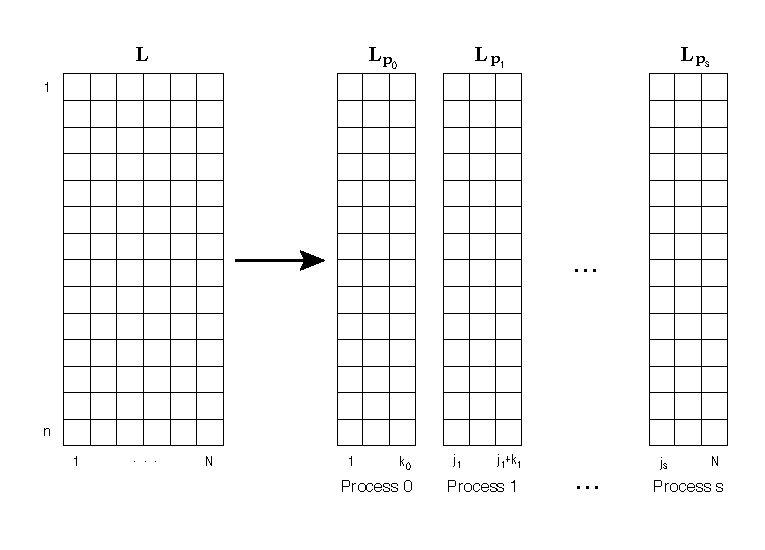
\includegraphics[width=0.8\textwidth]{figure/p91.pdf}
    \label{l_distribution}
    \caption{Distribution of the matrix $L$ into local sub-matrices $L_p$}
  \end{figure}

  \par \textcolor{red}{Parallelization of the $U$ computation}\\

  We focus in this part on the computation of the reduced covariance matrix $U$:\\
 $ U_{h+1} = U_h +  (H_{h+1}L_{h+1})^T R_{h+1}^{-1} H_{h+1}L_{h+1}$\\


  \begin{itemize}

\item The tangent observation operator is applied in parallel on each column of the local sub matrix $L_p$ (see Figure \ref{matrix_1}). The resulted matrix $HL_p$ is a sub-matrix of $HL$. The columns of $HL_p$ correspond to the same column indices as those available of matrix $HL_p$.

\begin{figure}[htpb]
        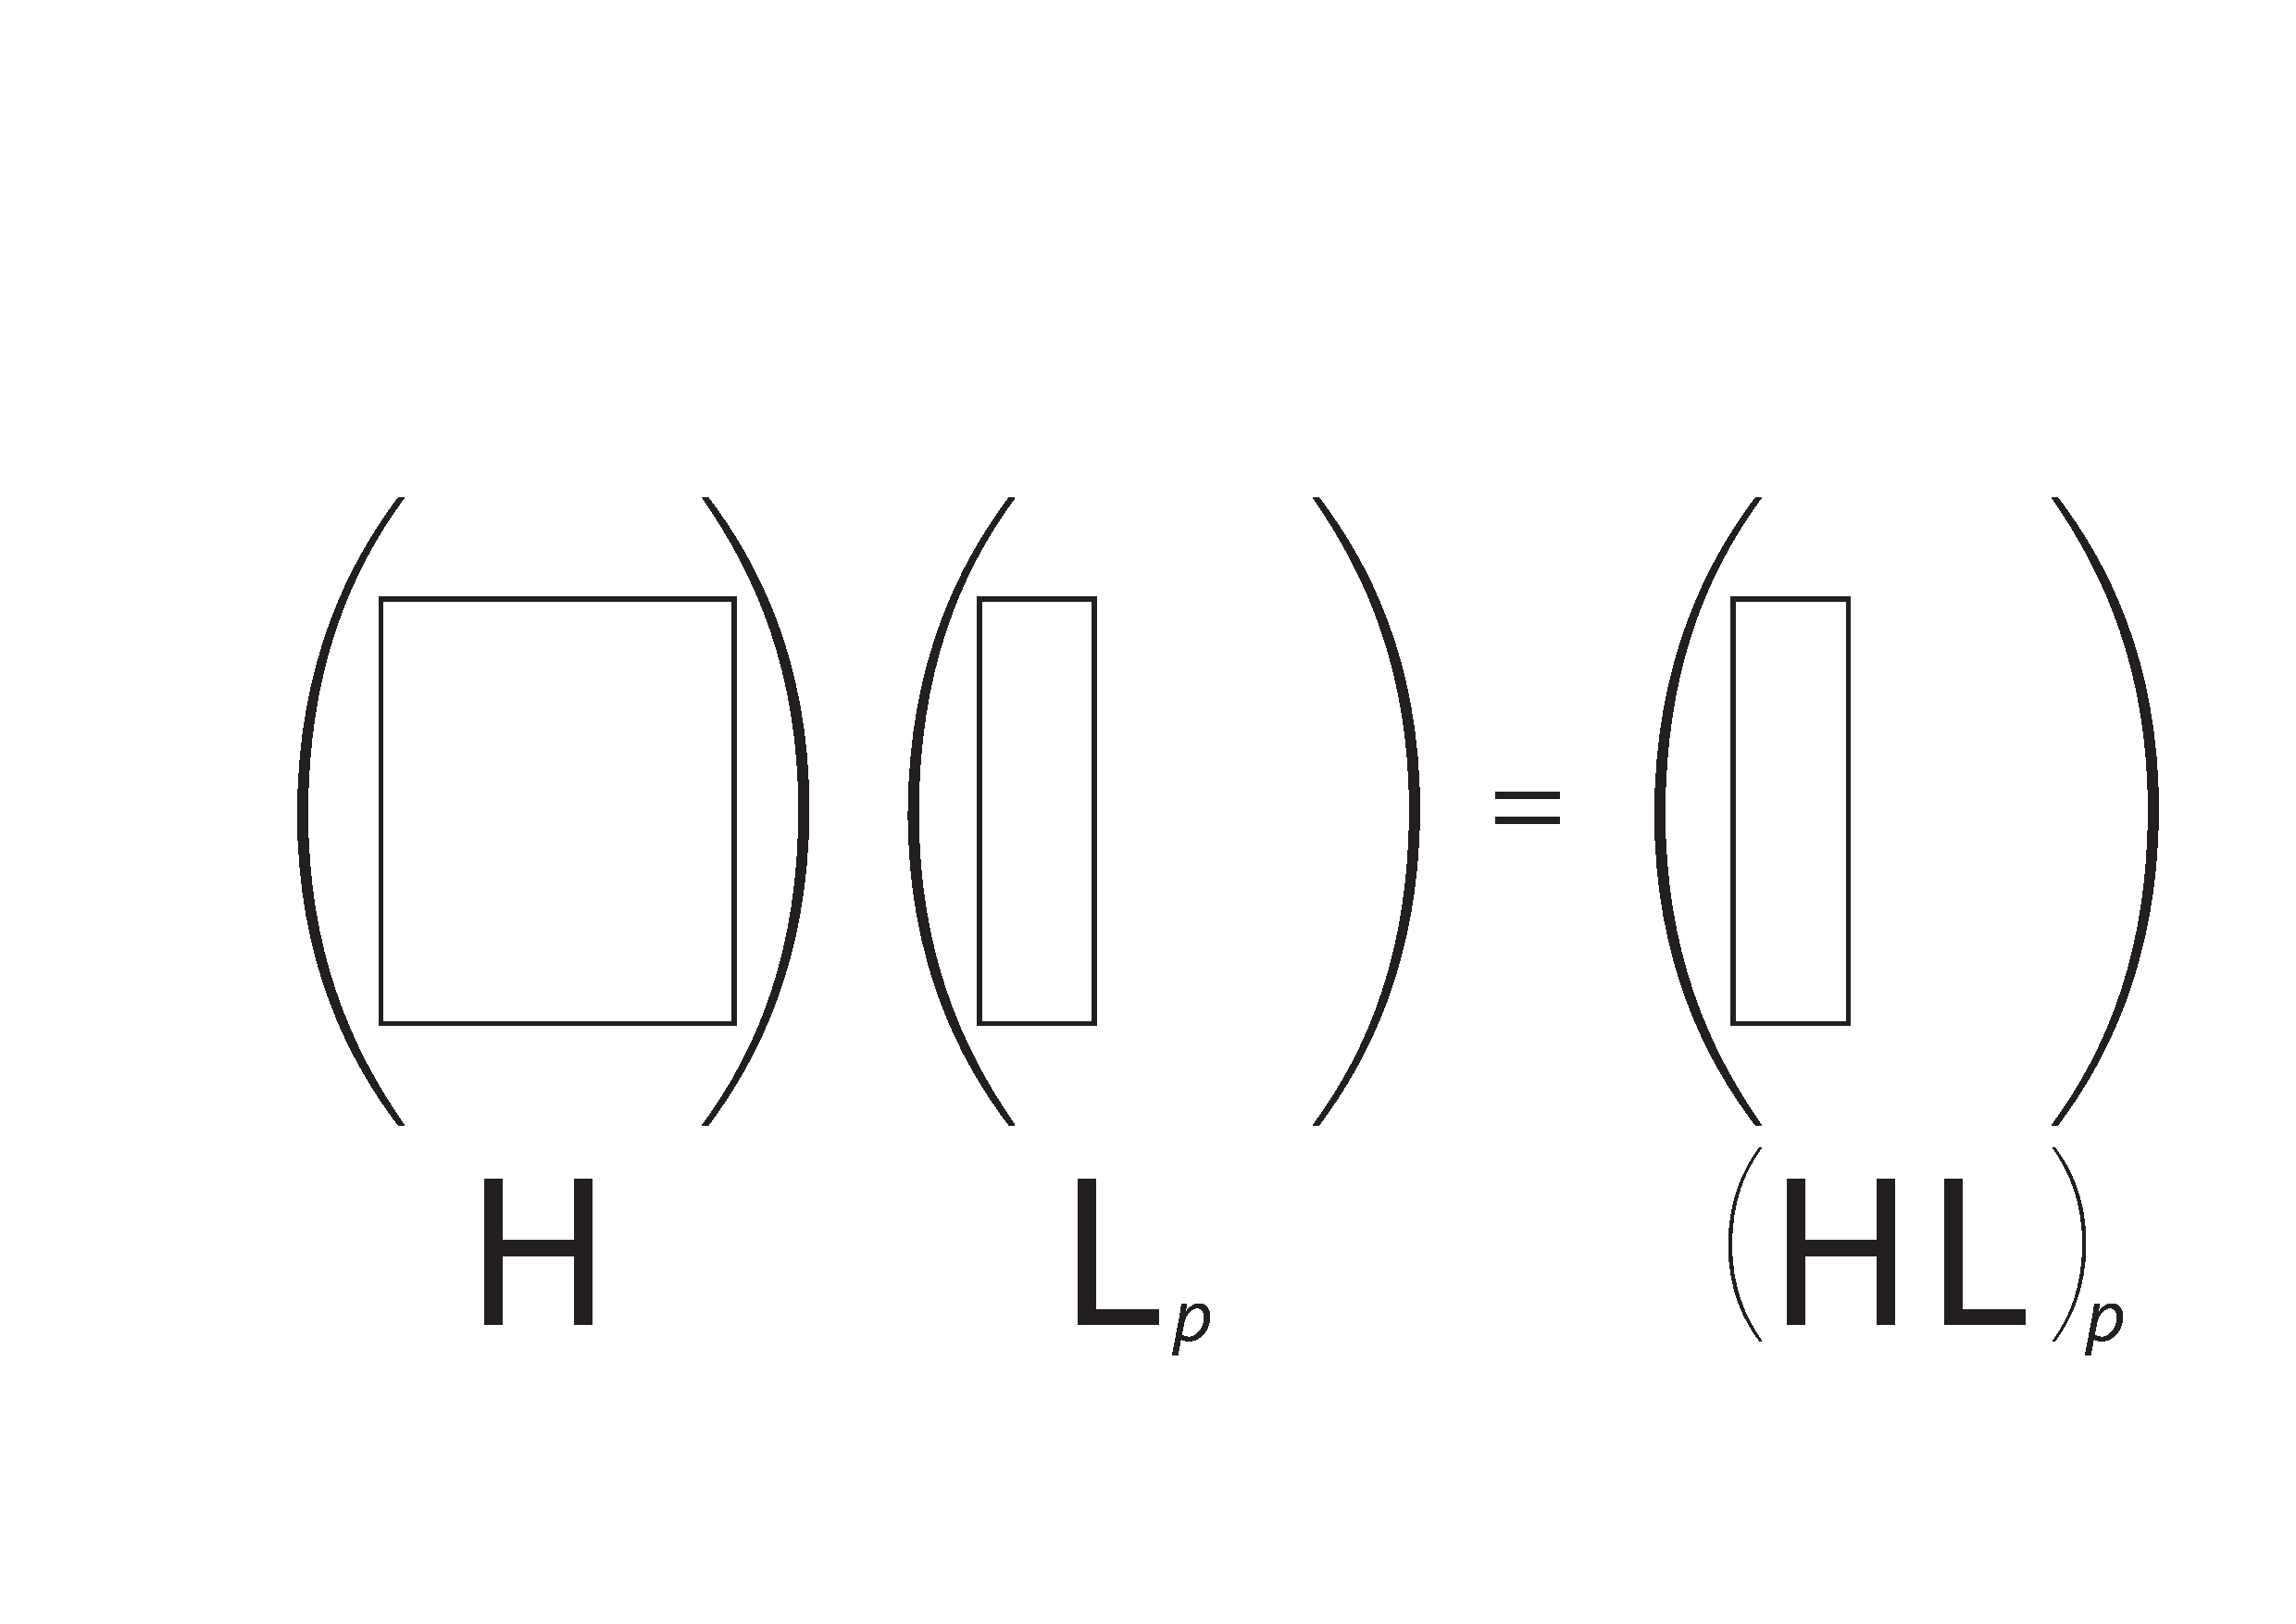
\includegraphics[width=0.6\textwidth]{figure/p92.pdf}
        \caption{Matrix-matrix product type 1}
        \label{matrix_1}
\end{figure}


\item Each process sends its local sub-matrix $HL_p$ to all others (allgather operation). Thus, each process owns the entire matrix  $HL$.\\

\item Each process computes the sub-matrix  $(R_{h+1}^{-1} H_{h+1}L_{h+1})_p$ of  $R_{h+1}^{-1} H_{h+1}L_{h+1}$ :\\
$(R_{h+1}^{-1} H_{h+1}L_{h+1})_p = R_{h+1}^{-1} (H_{h+1}L_{h+1})_p$ (see Figure \ref{matrix_1})

\item Each process computes the sub-matrix   $(U_{h+1})_p$  of  the reduced covariance matrix $U_{h+1}$:\\
 $ (U_{h+1})_p = (U_h)_p +  (H_{h+1}L_{h+1})^T (R_{h+1}^{-1} H_{h+1}L_{h+1})_p$ (see Figure \ref{matrix_1})

 \item Each process sends its local sub-matrix  $ (U_{h+1})_p$ to all others (allgather operation). Thus, each process owns the entire matrix  $U_{h+1}$.\\

\end{itemize}



\par \textcolor{red}{Parallelization of the $x^a$ computation}\\

Below is explained the update of the model state vector:\\
$ x_{h+1}^a = x_{h+1}^f + L_{h+1}U_{h+1}^{-1}(H_{h+1}L_{h+1})^T R_{h+1}^{-1} (y_{h+1}-H_{h+1}x_{h+1}^f)$\\


 \begin{itemize}
  \item Each process computes the innovation: $z = (y_{h+1}-H_{h+1}x_{h+1}^f)$.

  \item  The computation $d_p = (R_{h+1}^{-1}H_{h+1}L_{h+1})_p^Tz$  is performed in parallel by each process. Only $k_p$ rows of matrix  $(R^{-1}HL)^T$  are available locally (transpose of a matrix distributed by column). The innovation vector $z$ is fully allocated on each process. Consequently, each process is able to compute locally the $k_p$ elements of the vector $d$ whose indices correspond to those of the row of $(R^{-1}HL)^T$ available locally  (see \ref{matrix_2}).

  \item Each process sends its local sub-vector  $d_p$ to all others (allgather operation). Thus, each process owns the entire vector  $d$.\\

    \begin{figure}[htpb]
        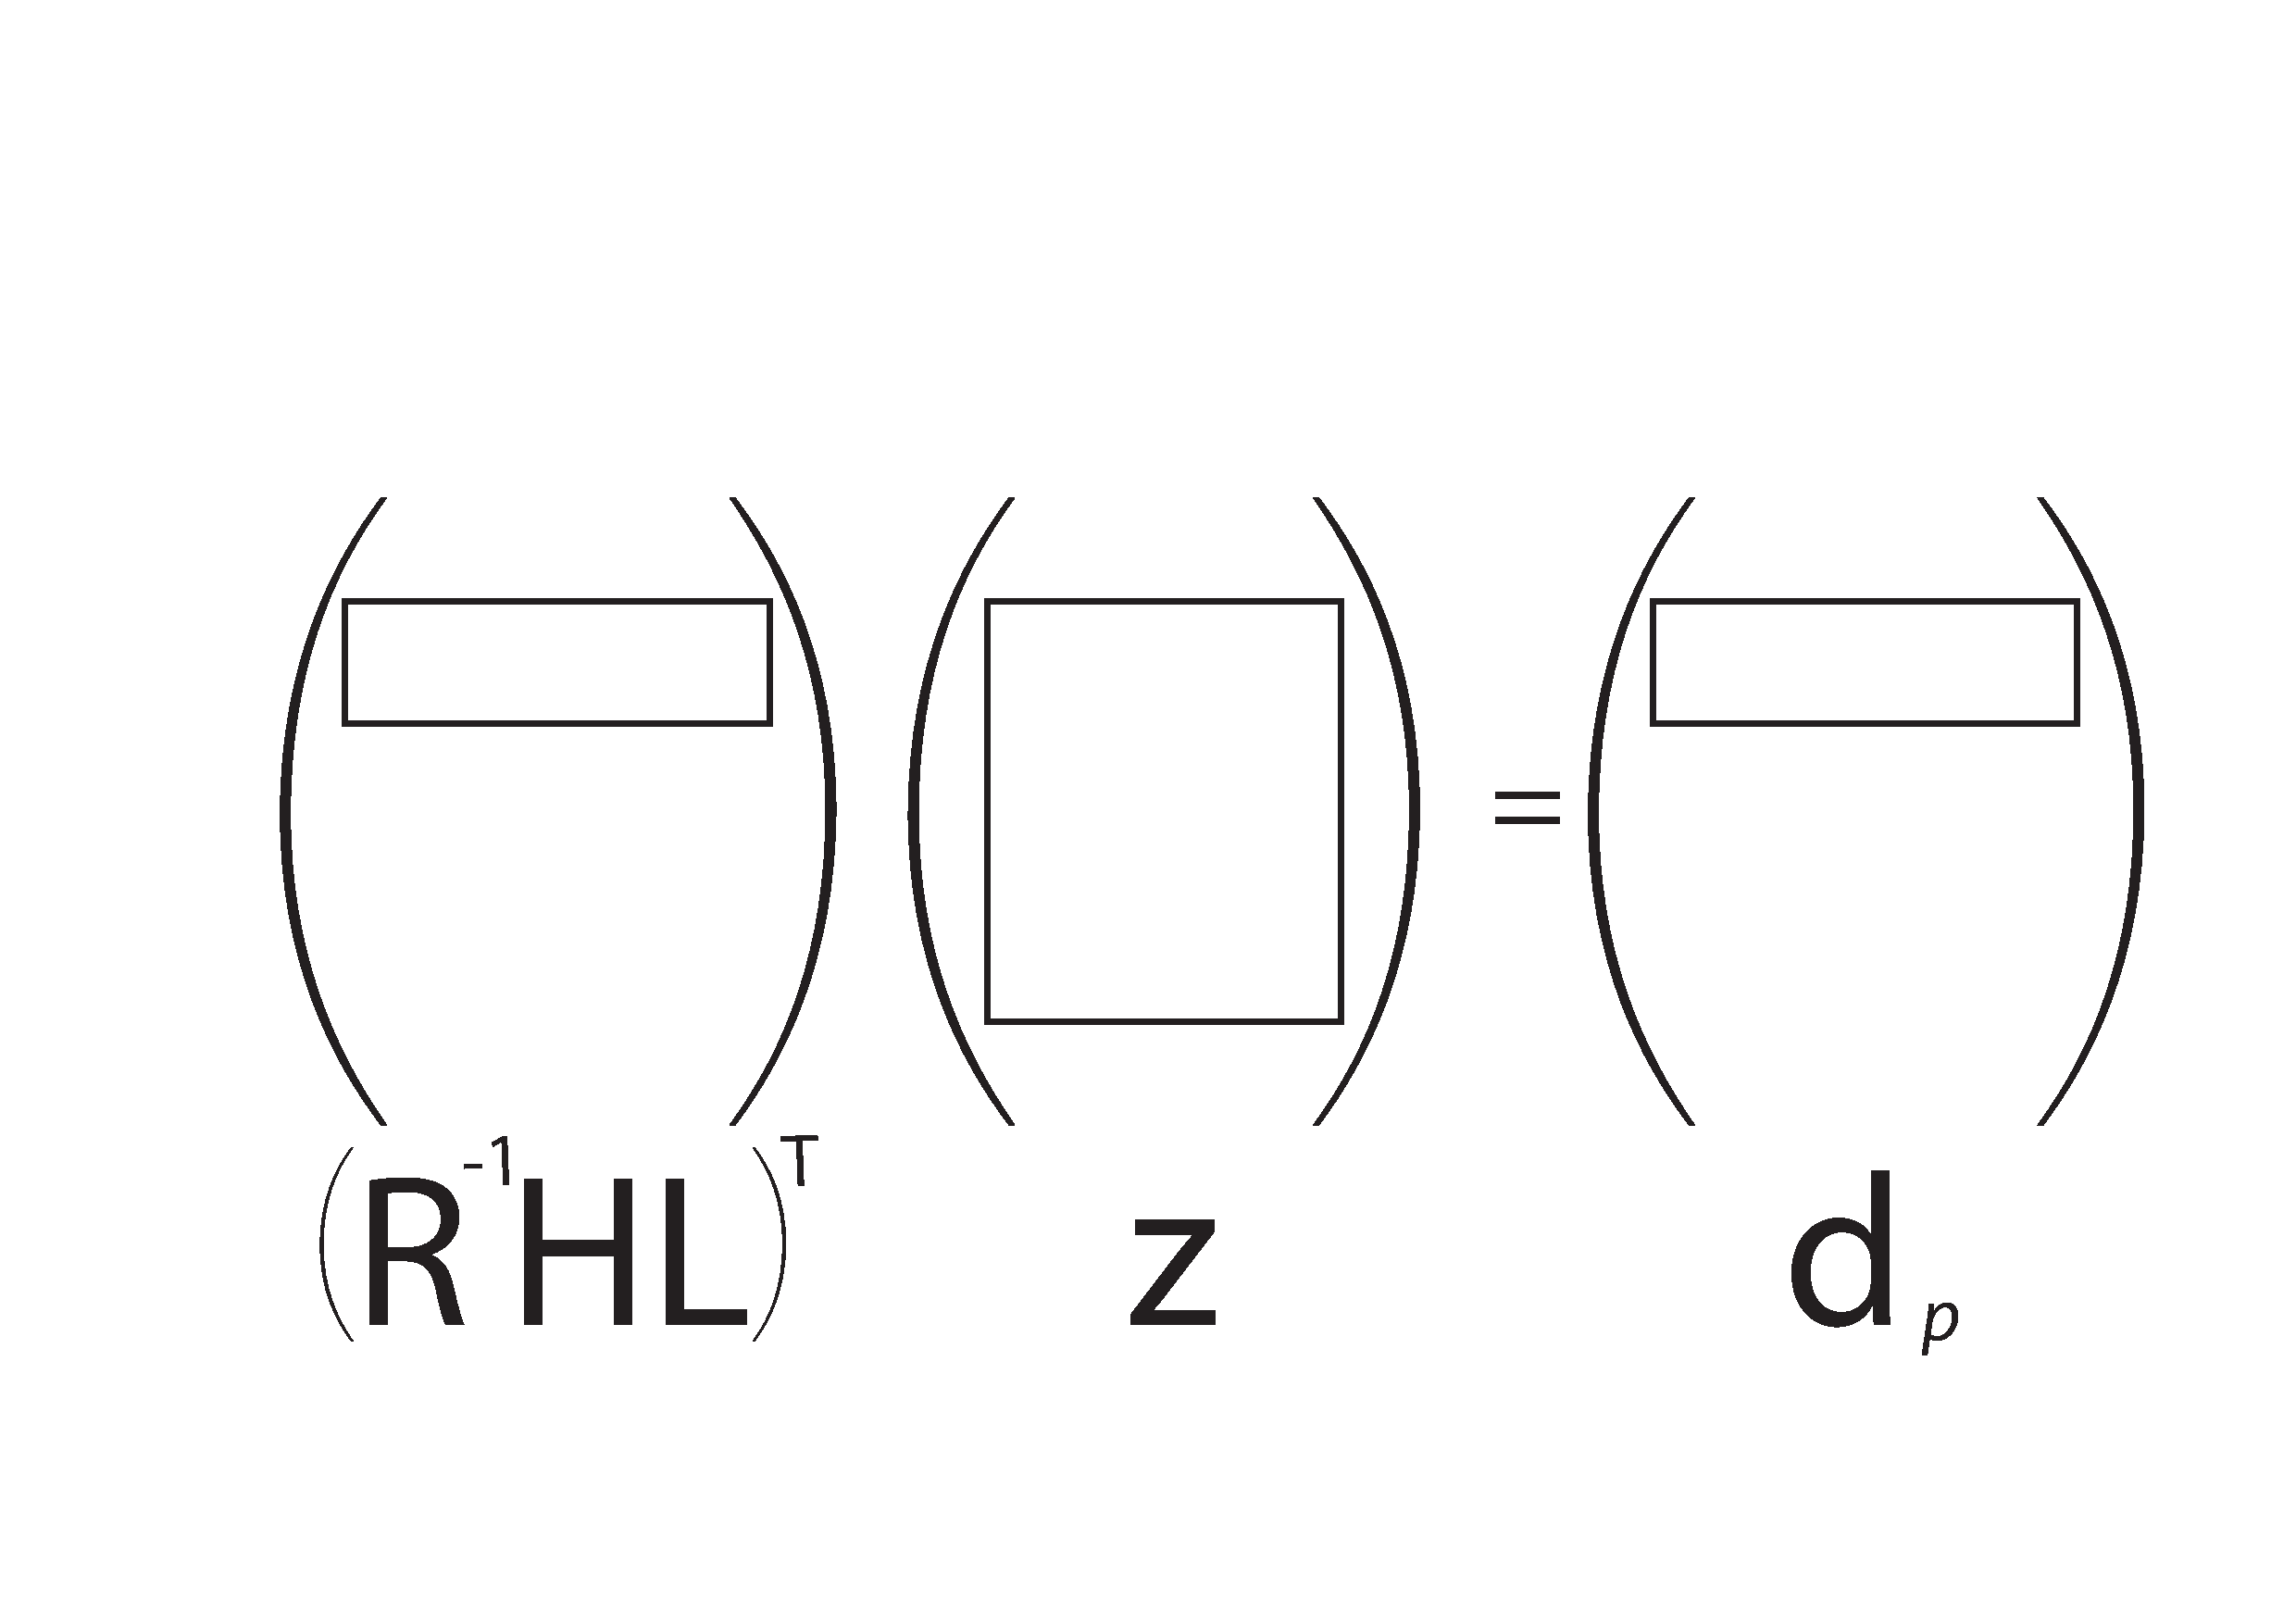
\includegraphics[width=0.6\textwidth]{figure/p93.pdf}
        \caption{Matrix-matrix product type 2}
        \label{matrix_2}
      \end{figure}

 \item The system  $U_{h+1}c = d$ is solved by each process.

  \item Each process computes computes the local contribution $\Delta x_p = (L_{h+1})_p c$ :\\
  Only $k_p$ columns of matrix $L_{h+1}$ and $k_p$ rows of vector $c$ are available locally. The product $\Delta x_p = (L_{h+1})_p c$ is a vector of the same size of $x^a$ which elements represent a partial sum of the product $L_{h+1} c$ (see Figure \ref{matrix_3}). Thus, to obtain the product  $L_{h+1} c$, the contribution of all the processes have to be summed (all reduce operation).

     \begin{figure}[htpb]
        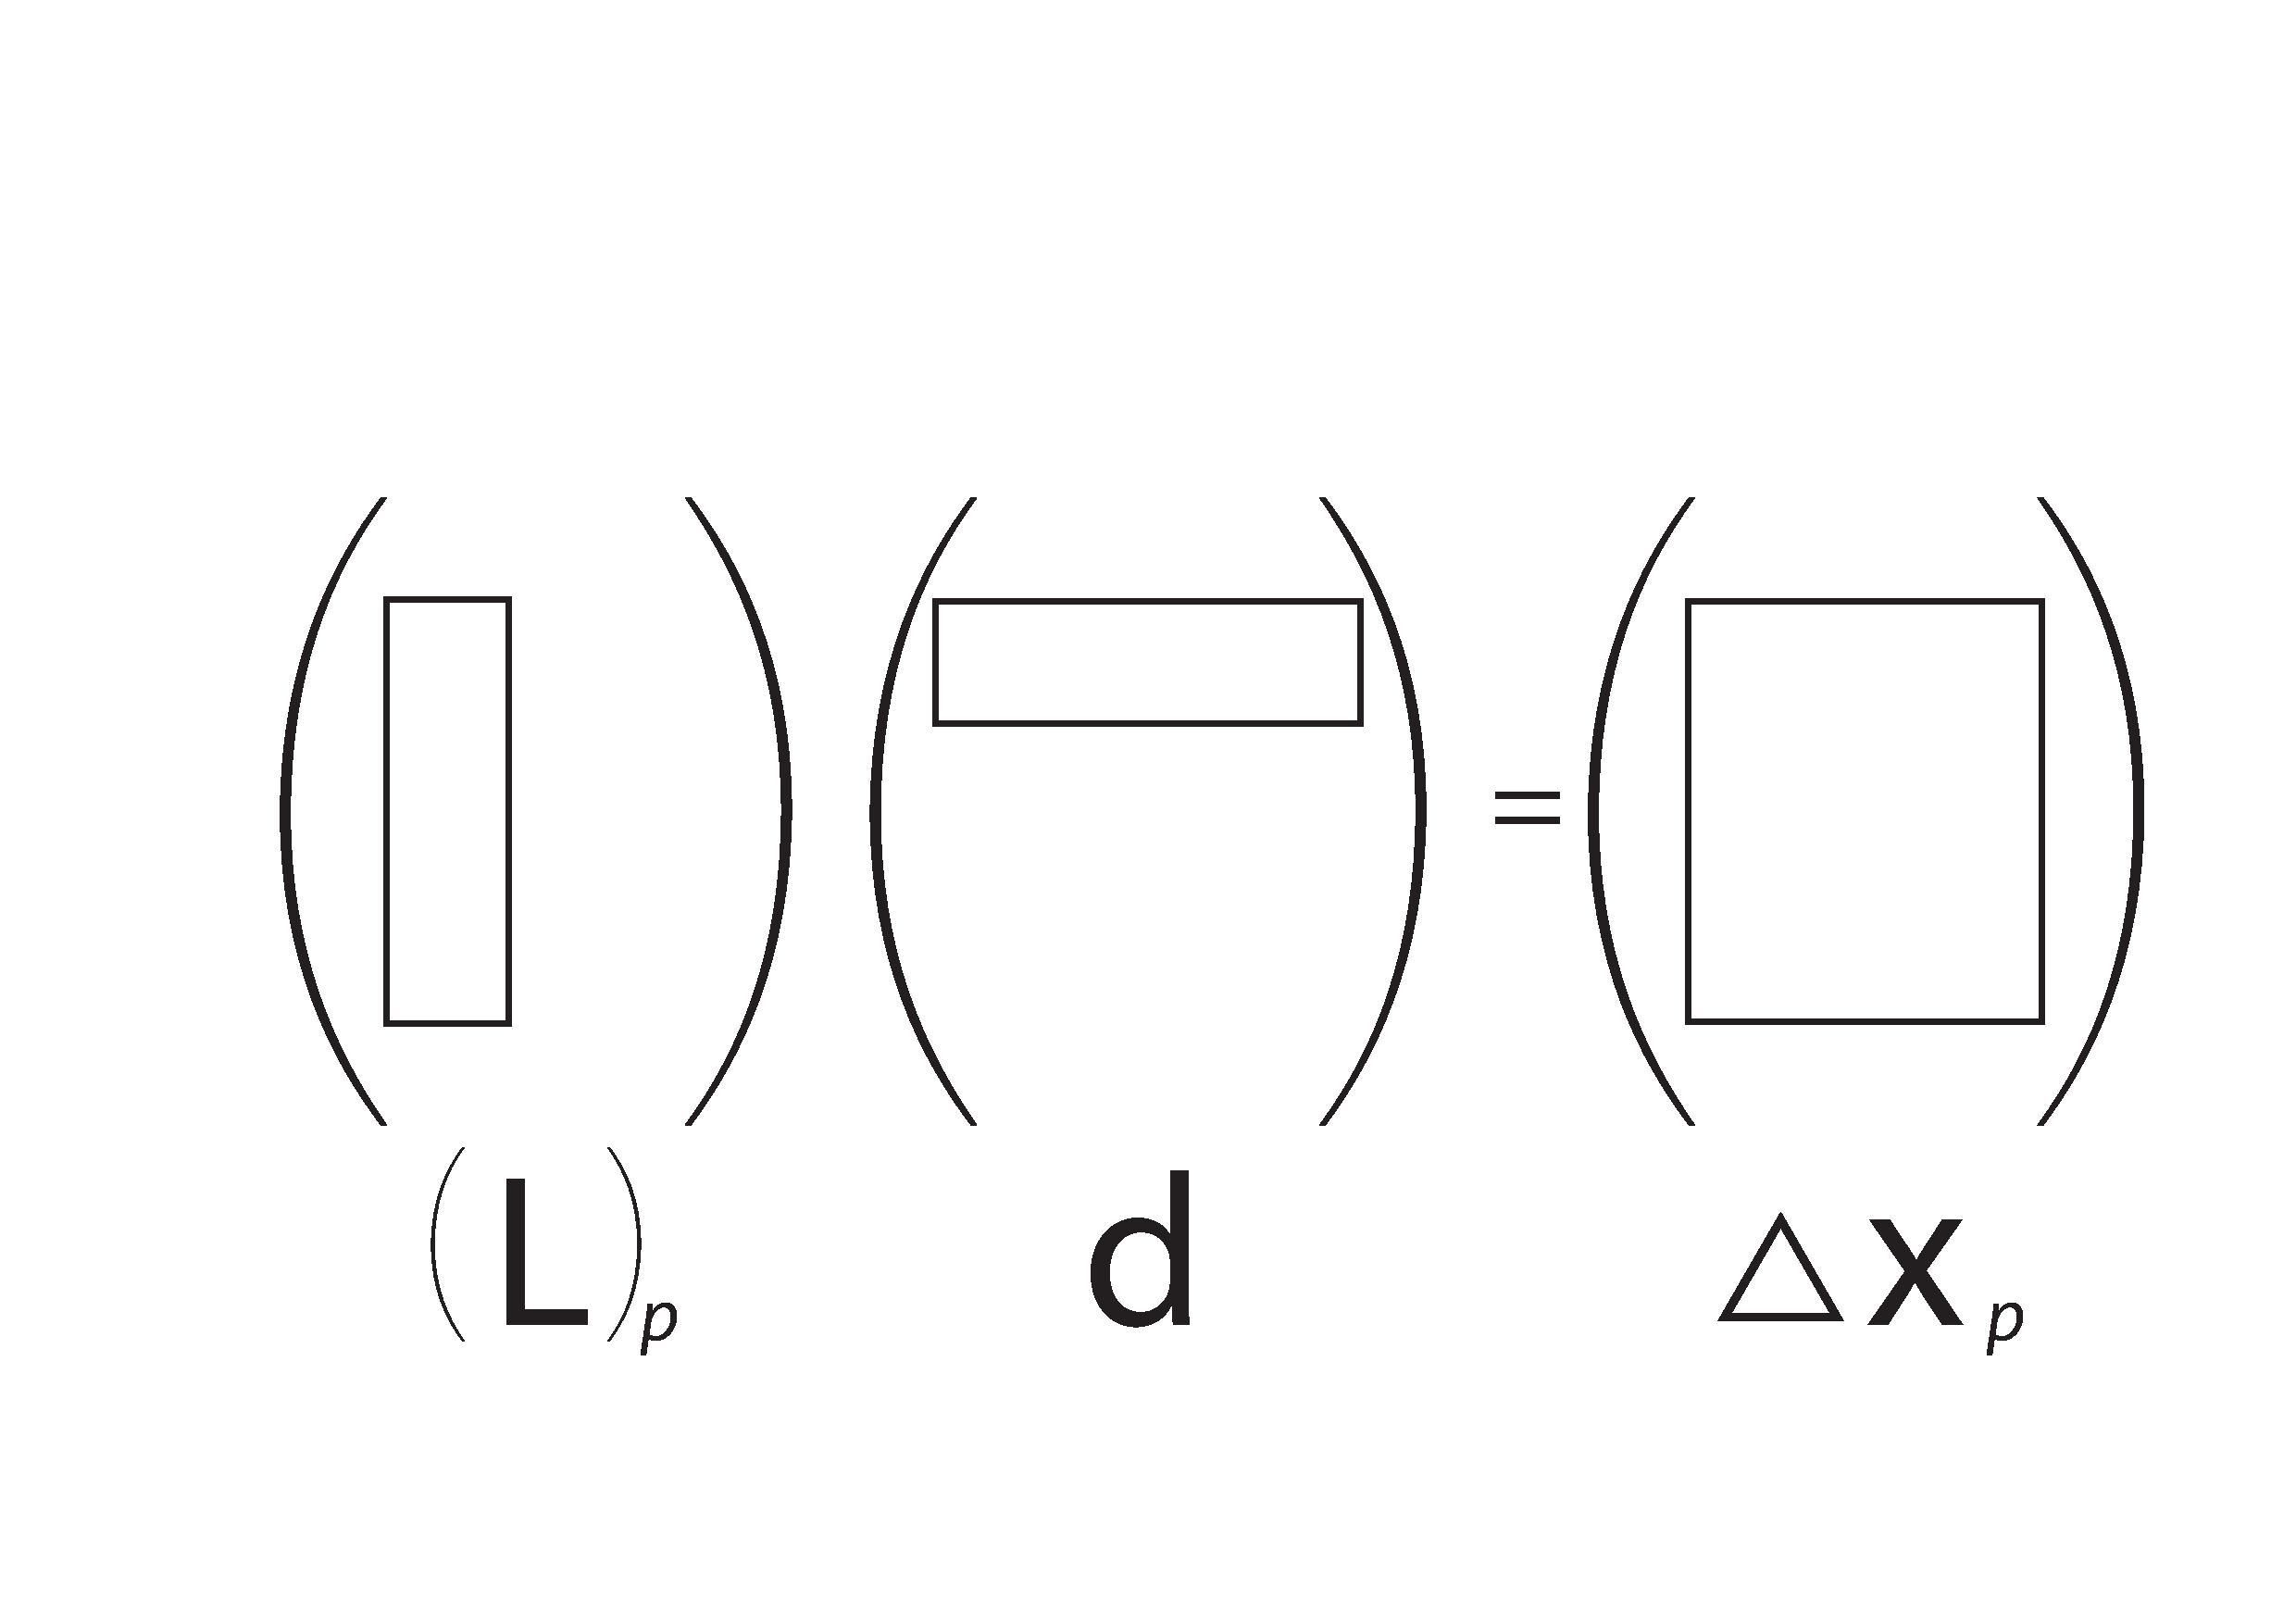
\includegraphics[width=0.6\textwidth]{figure/p94.pdf}
        \caption{Matrix-matrix product type 3}
        \label{matrix_3}
\end{figure}



  \end{itemize}


\hypertarget{par-seq-algo-roukf}{}\paragraph{Parallelization of the 'ReducedOrderUnscentedKalmanFilter'}\label{par-seq-algo-roukf}

  \par \textcolor{red}{Algorithm}\\


  \begin{DoxyEnumerate}
\item \-Sampling\-:
\begin{DoxyItemize}
\item $ C_{h} = \sqrt{U_h^{-1}} $\par

\item $ x_{h}^{(i)a} = x_h^a + L_hC_hI^{(i)} \textrm{, } \quad 1\leq i \leq p+1 $\par

\end{DoxyItemize}
\item \-Prediction\-:
\begin{DoxyItemize}
\item $ x_{h+1}^f = E_\alpha(\mathcal{M}_{h}(x_{h+1}^{(*)a})) $\par

\item $ x_{h+1}^{(i)f} = x_{h+1}^f + [\mathcal{M}_{h}(x_{h}^{*a}) - x_{h+1}^f]D_{\alpha}^{1/2} \Upsilon_p I^(i), \textrm{ resampling with SVD} $\par

\item $ L_{h+1} = [x_{h+1}^{(*)f}]D_\alpha [V^*]^T \in \mathcal{M}_{n,p} $\par

\item $ P_{h+1}^f = L_{h+1} (P_{\alpha}^V)^{-1} L_{h+1}^T $
\end{DoxyItemize}
\item \-Update\-:
\begin{DoxyItemize}
\item $ [\tilde{y}] = [\mathcal{H}_{h+1}(x_{h+1}^{(*)f}) - E_\alpha(\mathcal{H}_{h+1}(x_{h+1}^{(*)f})) ]$\par

\item $ D_m = [\tilde{y}]^T R_{h+1}^{-1}[\tilde{y}] \in \mathcal{M}_r $\par

\item $ U_{h+1} = P_{\alpha}^V + [V^*] D_\alpha \bigl(1 + D_m(D_\alpha - D_V)\bigr)^{-1} D_m D_\alpha [V^*]^T \in \mathcal{M}_{p} $\par

\item $ \{HL\}_{h+1} = [\tilde{y}]( 1 + D_\alpha D_m)^{-1}\Bigl(1 + D_V \bigl( 1+D_m (D_\alpha-D_V) \bigr)^{-1} D_m \Bigr) D_\alpha[V^*]^T $\par

\item $ x_{h+1}^a = x_{h+1}^f + L_{h+1}U_{h+1}^{-1}\{HL\}_{h+1}^T R_{h+1}^{-1} (y_{h+1}-E_\alpha(y_{h+1}^{(*)}))$\par

\item $ P_{h+1}^a = L_{h+1} U_{h+1}^{-1} L_{h+1}^T$
\end{DoxyItemize}
\end{DoxyEnumerate}\-With\-: \par
 $x_h^f$ forecast state vector; \par
 $x_h^a$ analysis state vector; \par
 $y_h$ observation vector; \par
 $\mathcal{H}_h$ observation operator that maps the state space to the observation space; \par
 $H_h$ observation operator linearized at $x^f_h$; \par
 $P^f_h$ error covariance matrix of $x_h^f$; \par
 $P^a_h$ error covariance matrix of $x_h^a$; \par
 $R_h$ observational error covariance matrix; \par
 $\mathcal{M}_h$ model.



 \begin{itemize}
  \item  The particles  $x_{h}^{(i)a}$ are distibuted over the processes.
  \item Each process executes the sequential ROUKF algorithm with its local particles.
  \item The matrices $x_{h+1}$, $L_{h+1}$, $(HL)_{h+1}$ et $U_{h+1}$ are updated with the different parallel matrix-matrix products presented in Section \ref{par-seq-algo-roekf}.
  \end{itemize}


\hypertarget{par-seq-example}{}\subsection{Example Programs}\label{par-seq-example}


The examples are located in the {\ttfamily example/clamped\_bar} directory.\footnote{To have a summary of \emph{Verdandi} contents see Section \ref{overview}.}


\hypertarget{par-seq-example-compilation}{}\paragraph{Compilation}\label{par-seq-example-compilation}

First of all, the preprocessor variable $ VERDANDI\_WITH\_MPI $ has to be defined in files  \textbf{reduced\_order\_extended\_kalman\_filter.cpp} and \textbf{reduced\_order\_unscented\_kalman\_filter.cpp}:

\begin{frame_cpp}
#define VERDANDI_DEBUG_LEVEL_4
#define SELDON_WITH_BLAS
#define SELDON_WITH_LAPACK

#define VERDANDI_WITH_ABORT
#define VERDANDI_DENSE

#define VERDANDI_WITH_MPI

#if defined(VERDANDI_WITH_MPI)
#include <mpi.h>
#endif


#include "Verdandi.hxx"
#include "seldon/SeldonSolver.hxx"

#include "model/ClampedBar.cxx"
#include "observation_manager/LinearObservationManager.cxx"
#include "method/ReducedOrderUnscentedKalmanFilter.cxx"


int main(int argc, char** argv)
{

    VERDANDI_TRY;

    ...
}
\end{frame_cpp}

Then, compile the program \textbf{generate\_observation.cpp}:


\begin{frame_bash}
$ scons generate_observation
\end{frame_bash}

Finally, compile the programs \textbf{reduced\_order\_extended\_kalman\_filter.cpp} and \textbf{reduced\_order\_unscented\_kalman\_filter.cpp}  with the option 'mpi=yes':
\begin{frame_bash}
$ scons reduced_order_extended_kalman_filter mpi=yes
$ scons reduced_order_unscented_kalman_filter mpi=yes
\end{frame_bash}



\hypertarget{par-seq-example-observation}{}\paragraph{Observation}\label{par-seq-example-observation}

\-Since no observations are given yet, we have to generate some. \-Execute the following command\-:
\begin{frame_bash}
host<~/> ./generate_observation configuration/truth.lua
\end{frame_bash}
  to run the model with the initial conditions described in {\ttfamily truth.\-lua}, without data assimilation. \-This should generate a result file ({\ttfamily truth-\/state\-\_\-forecast.\-bin}) in the directory {\ttfamily example/clamped\-\_\-bar/result/}. \-This file store the state (displacement, velocity, $ \theta_{f} $) trajectory.

\-The generated state (displacement, velocity, $ \theta_{f} $) will serve as observations for the assimilation.



\hypertarget{par-seq-example-dam}{}\paragraph{Data Assimilation with ROEKF and ROUKF}\label{par-seq-example-dam}


\-To use the \hyperlink{reduced_order_extended_kalman_filter}{\-Reduced \-Order \-Extended \-Kalman \-Filter} and the \hyperlink{reduced_order_unscented_kalman_filter}{\-Reduced \-Order \-Unscented \-Kalman \-Filter} methods, execute the following commands.
\begin{frame_bash}
$ mpirun -n 2 reduced_order_extended_kalman_filter configuration/assimilation.lua
$ mpirun -n 2 reduced_order_unscented_kalman_filter configuration/assimilation.lua
\end{frame_bash}
  \-This runs the model with the initial conditions described in {\ttfamily example/clamped\-\_\-bar/configuration/assimilation.\-lua}. \-The simulation begins with erroneous values for the parameter $ \theta_f $. \-This should generate the same results as for the sequential simulation.\\


  \textbf{Warning:}  The number of processes should be less than or equal to the size of the reduced model state vector.



\hypertarget{par-seq-performance}{}\subsection{Performance}\label{par-seq-performance}

The figures \ref{titre2} and \ref{titre3} introduce the resulting performance of the ROEKF and ROUKF algorithms applied to the sequential model ClampedBar. These simulations were performed on 2 x 3 GHz Quad-Core Intel Xeon with a 16 GB of memory in which the processes used during simulation were placed at arbitrary cores relative to the process constructing the network.

\begin{figure}
    \caption{\label{titre2} Speed up of the parallel ROEKF algorithm applied to the sequential model ClampedBar with $N_{state} = 10^4$, $N_{observation} = 10^2$ and $N_{sigma\_point} = 16$.}

 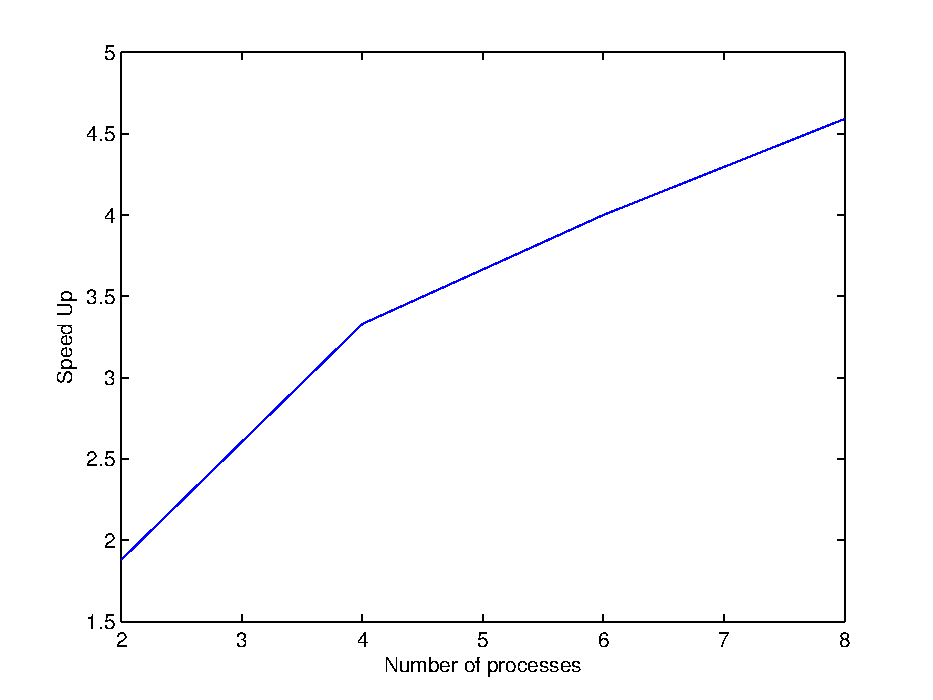
\includegraphics[width=0.8\textwidth]{figure/speed_up_roekf.pdf}

   \end{figure}



 \begin{figure}
  \caption{\label{titre3} Speed up of the parallel ROUKF algorithm applied to the sequential model ClampedBar with $N_{state} = 10^4$, $N_{observation} = 10^2$ and $N_{sigma\_point} = 16$.}

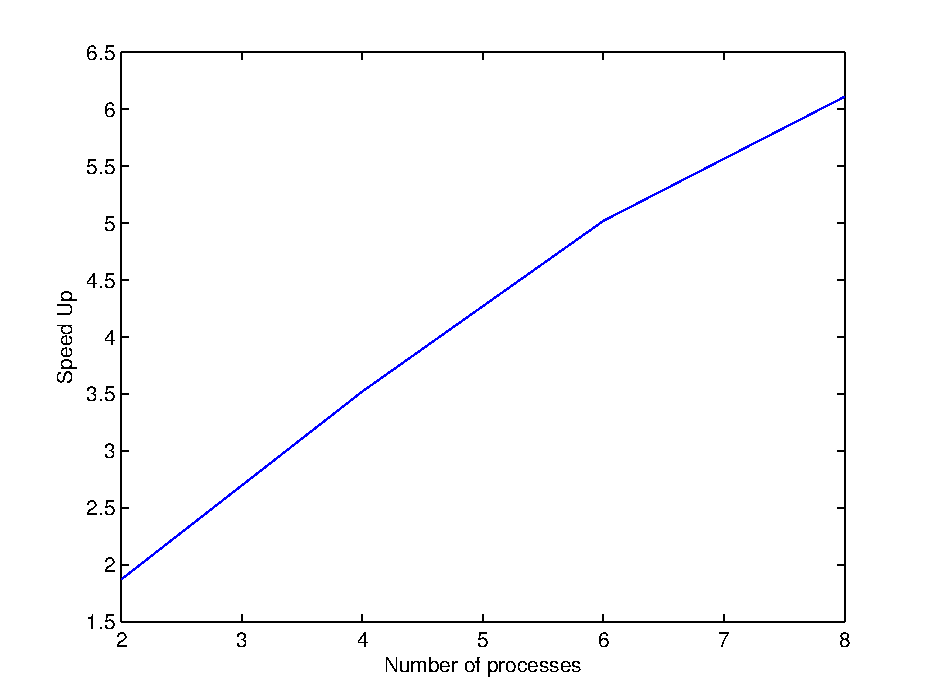
\includegraphics[width=0.8\textwidth]{figure/speed_up_roukf.pdf}

\end{figure}


\newpage


\hypertarget{seq-par}{}\section{Sequential Method applied to Parallel Model}\label{seq-par}

Verdandi intends to provide the ability to apply its data assimilation methods to models whose state vector is distributed on several processes. In the case of large scale state vector, neither the model nor the data assimilation method can afford to allocate a variable of this size. Consequently, several data assimilation variables
could be distributed, for instance the sensitivity matrix and the variance. The number of components to be stored locally has to be compatible with the distributed model state vector for parallel matrix-vector operations.

The management of the types in Verdandi, detailed in Section \ref{seq-par-type}, enabled to implement this capability easily. The chosen solution was to create an interface between Seldon, the linear algebra library used in Verdandi, and PETSc a framework for parallel computing. This choice do not confine the type of the model state vector only to PETSc distributed structures since any MPI distributed structures can be encapsulated or copied in a PETSc object.


\hypertarget{seq-par-type}{}\subsection{Types Management in Verdandi}\label{seq-par-type}


The implementation of the Verdandi algorithms relies on the linear algebra library Seldon. This library provides different matrix and vector structures, and many functions for computations (linear algebra). It provides matrices for two main categories: dense matrices and sparse matrices. Among dense matrices, there are specific structures for rectangular matrices, symmetric matrices, hermitian matrices and triangular matrices. Each type includes several formats: rectangular dense matrices may be stored by rows or by columns; symmetric dense matrices may be stored as rectangular matrices or only upper part of the matrix is stored. Many different types
for sparse matrix are also available. All  of these matrix classes share the same interface. Linear algebra computation functions are template functions and many BLAS operations bringing into play different matrix types are implemented.


Example program which computes the product of a dense matrix by a sparse matrix:


\begin{frame_cpp}
// Dense  matrix.
Matrix<double, General, RowMajor> A(3, 3), C(3, 3);
A.Fill();
C.Fill();
// Sparse matrix.
Matrix<double, General, ArrayRowSparse> B(3, 3);
B(0, 0) = 2.0;
B(1, 0) = 1.0;
// Computes matrix-matrix product alpha*A*B + beta*C -> C.
// This function is overloaded for all types of matrices.
MltAdd(1.0, A, B, 2.0, C);
\end{frame_cpp}


In Verdandi, the model and the observation manager can provide their vector and matrix types to the data assimilation method thanks to the C++ 'typedef' mechanism. For instance :


\begin{frame_cpp}
class Model
{
    public:
        //! Type of the state error variance.
        typedef Matrix<double, General, RowSparse> state_error_variance;
        /*! \brief Type of the reduced matrix \f$U\f$ in the \f$LUL^T\f$
        decomposition of the state error variance. */
        typedef Matrix<double, General, RowMajor> state_error_variance_reduced;
        //! Type of the state vector.
        typedef Vector<double> state;
	...
}
\end{frame_cpp}


\begin{frame_cpp}
class ObservationManager
{
    public:
        //! Type of the tangent linear operator.
        typedef Matrix<double, General, RowSparse> tangent_linear_operator;
        //! Type of the observation vector.
        typedef Vector<double> observation;
	...
}
\end{frame_cpp}


Thus, the data assimilation method is able to get back the type of the object to instantiate. For instance, to fetch the type of the model state vector:

\begin{frame_cpp}
template <class Model, class ObservationManager>
class DataAssimilationMethod
{
...
        //! Type of the model state vector.
        typedef typename Model::state model_state;
...
}
\end{frame_cpp}



\hypertarget{seq-par-ds}{}\subsection{Distributed Structure in Seldon}\label{seq-par-ds}


To ensure the compatibility of the Verdandi data assimilation methods with distributed models,  it was sufficient to:

\begin{itemize}

\item add vector and matrix distributed structures to Seldon.

\item implement the linear algebra computation functions for these new types, required by the concerned data assimilation methods.

\end{itemize}

\hypertarget{seq-par-ds-vector}{}\paragraph{Distributed Vector}\label{seq-par-ds-vector}


The class Seldon$::$Vector$<$double, PETScPar$>$  encapsulate a distributed PETSc vector of type \textbf{VecMPI} . This class implement the same interface as a classic Seldon vector. The whole set of BLAS1 operations have been implemented for this type.

The source files of the class Seldon$::$Vector$<$double, PETScPar$>$  are located in the seldon/vector/ directory. Several methods are specific of  Seldon$::$Vector$<$double, PETScPar$>$ class:

\begin{frame_cpp}
template <class T, class Allocator>
class Vector<T, PETScPar, Allocator>: public PETScVector<T, Allocator>
{
	...

    // Returns a reference on the inner petsc vector.
    Vec& GetPetscVector();

    // Returns a const reference on the inner petsc vector.
    const Vec& GetPetscVector() const;

    // Sets the MPI communicator.
    void SetCommunicator(MPI_Comm mpi_communicator);

    // Inserts or adds values into certain locations of a vector.
    // \warning These values may be cached, so 'Flush' must be called after
    // all calls to SetBuffer() have been completed.
    void SetBuffer(int i, T value, InsertMode insert_mode = INSERT_VALUES);

    // Assembles the PETSc vector.
    void Flush();

    // Returns the range of indices owned by this processor.
    // The vectors are laid out with the first \f$n_1\f$ elements on the first
    // processor, next \f$n_2\f$ elements on the second, etc. If the current
    // processor is \f$k\f$, this method returns \f$n_k\f$ in \a i and
    // \f$n_{k+1}\f$ in \a j. If \a i is set to PETSC_NULL on entry, it is not
    // modified by this function. Same is true for \a j.
    void GetProcessorRange(int& i, int& j) const;

    ...
}
\end{frame_cpp}


\par These specific methods may be necessary during the construction of a distributed vector. These methods are never called by data assimilation methods which delegate the distributed variable initializations to models and observation managers.


\textbf{Distributed PETSc vector example program}


\begin{frame_cpp}

    Vec x, y;

    int N = 10;

    ierr = VecCreateMPI(PETSC_COMM_WOLRD, N, &x); CHKERRQ(ierr);
    ierr = VecCreateMPI(PETSC_COMM_WOLRD, N, &y); CHKERRQ(ierr);
    ierr = VecSet(x, 3.0); CHKERRQ(ierr);
    ierr = VecSet(y, 1.0); CHKERRQ(ierr);

    ierr = VecAssemblyBegin(x); CHKERRQ(ierr);
    ierr = VecAssemblyEnd(x); CHKERRQ(ierr);
    ierr = VecAssemblyBegin(y); CHKERRQ(ierr);
    ierr = VecAssemblyEnd(y); CHKERRQ(ierr);

    ierr = VecAXPY(y, -1.0, x); CHKERRQ(ierr);

    ierr = VecDestroy(&x); CHKERRQ(ierr);
    ierr = VecDestroy(&y); CHKERRQ(ierr);


\end{frame_cpp}


\textbf{The same example using the Vector$<$double, PETScPar$>$ class}

\begin{frame_cpp}

    Vector<double, PETScPar> x, y;
    x.Reallocate(10);
    y.Reallocate(10);
    x.Fill(3.);
    y.Fill(1.);

    Add(-1., x, y);

\end{frame_cpp}


\hypertarget{seq-par-ds-dmatrix}{}\paragraph{Distributed Dense Matrix}\label{seq-par-ds-dmatrix}


The class Seldon$::$Matrix$<$T, Prop, PETScMPIDense, Allocator$>$  encapsulate a  dense distributed PETSc matrix of type \textbf{MATMPIDENSE} . This class implement the same interface as a classic Seldon matrix.

The source files of the class Seldon$::$Matrix$<$T, Prop, PETScMPIDense, Allocator$>$   are located in the seldon/matrix/ directory. Several methods are specific of  Seldon$::$Matrix$<$T, Prop, PETScMPIDense, Allocator$>$  class:


\begin{frame_cpp}
template <class T, class Prop, class Allocator>
class Matrix<T, Prop, PETScMPIDense, Allocator>:
public PetscMatrix<T, Prop, RowMajor, Allocator>
{
	...

    // Returns a reference on the inner petsc matrix.
    Mat& GetPetscMatrix();
    // Returns a const reference on the inner petsc matrix.
    const Mat& GetPetscMatrix() const;


    // Sets the MPI communicator.
    void SetCommunicator(MPI_Comm mpi_communicator);
    // Returns the MPI communicator of the current PETSc matrix.
    MPI_Comm GetCommunicator() const;

    // Inserts or adds values into certain locations of a matrix.
    // \warning These values may be cached, so 'Flush' must be called after all
    // calls to SetBuffer() have been completed.
    void SetBuffer(int, int, T, InsertMode);

    // Assembles the PETSc matrix.
    void Flush() const;

    // Returns the range of row indices owned by this processor.
    // The matrix is laid out with the first \f$n_1\f$ rows on the first
    // processor, next \f$n_2\f$ rows on the second, etc. If the current
    // processor is \f$k\f$, this method returns \f$n_k\f$ in \a i and
    // \f$n_{k+1}\f$ in \a j. If \a i is set to PETSC_NULL on entry, it is not
    // modified by this function. Same is true for \a j.
    void GetProcessorRowRange(int& i, int& j) const;

    ...
}
\end{frame_cpp}


\par These specific methods may be necessary during the construction of a distributed matrix. These methods are never called by data assimilation methods which delegate the distributed variable initializations to models and observation managers.

\hypertarget{seq-par-ds-smatrix}{}\paragraph{Distributed Sparse Matrix}\label{seq-par-ds-smatrix}

The class Seldon$::$Matrix$<$T, Prop, PETScMPIAIJ, Allocator$>$  encapsulate a sparse distributed PETSc matrix of type \textbf{MATMPIAIJ} . This class has the same interface as the  Seldon$::$Matrix$<$T, Prop, PETScMPIDense, Allocator$>$ class  introduced previously.

The source files of the class Seldon$::$Matrix$<$T, Prop, PETScMPIAIJ, Allocator$>$   are located in the seldon/matrix/ directory



\hypertarget{seq-par-dm}{}\subsection{'PETScClampedBar' Distributed Model}\label{seq-par-dm}


Verdandi provides an implementation of the 'ClampedBar' model based on the distributed structures available in Seldon. The source files of the distributed 'PetscClampedBar' model are located in the verdandi/model/ directory.



\hypertarget{seq-par-dm-m}{}\paragraph{The 'PETScClampedBar' Model}\label{seq-par-dm-m}


The clamped bar model describes the vibration of a bar clamped at one end. The bar is discretized with $Nx$ finite elements of the same length. With the hypothesis of "small displacements", it follows the linear system:

\begin{center} $ M \ddot Y + C \dot Y + K Y = F_{\theta_f}$ \par
 \end{center}

 where $M$  is the mass matrix, $K$  is the stiffness matrix,  $C$  is the damp matrix and  $F(\theta_f) = \sin(\frac{\pi t}{t_f}) M_{\theta_f} (1 ... 1)^T$  is the effort vector.


 The clamped bar model is solved numerically using a Newmark scheme (middle point) for integration in time:

 $ \ddot Y_{h + \frac{1}{2}} = \frac{\ddot Y_{h+1} + \ddot Y_{h} }2 = \frac{\dot Y_{h+1} - \dot Y_{h} } {\Delta t} $ \par
$ \dot Y_{h + \frac{1}{2}} = \frac{\dot Y_{h+1} + \dot Y_{h} }2 = \frac{Y_{h+1} - Y_{h} } {\Delta t} $\\


Algorithmically, it follows:

$ \dot Y_{h + 1} = \frac{2}{\Delta t}(Y_{h+1} - Y_{h}) - \dot Y_{h} $ \par
$Newmark_1 = \frac{1}2K + \frac{1}{\Delta t}C + \frac{2}{\Delta t^2}M$ \par
$Newmark_0 = -\frac{1}2 K + \frac{1}{\Delta t}C + \frac{2}{\Delta t^2}M$ \par
$Newmark_1Y_{h+1} = Newmark_0Y_{h} + \frac{2}{\Delta t}M\dot Y_{h} + F_{h + \frac{1}{2}}(\theta_f)$\\

The matrices  $M$, $Newmark_0$ and $Newmark_1$ are sparse distributed matrices of type Matrix$<$T, Prop, PETScMPIAIJ, Allocator$>$. The effort vector $F$ is a distributed vector of type  Vector$<$double, PETScPar$>$:


\begin{frame_cpp}
template <class T>
class PetscClampedBar: public VerdandiBase
{
    public:

    ...

    //! Mass matrix.
    Matrix<T, General, PETScMPIAIJ> mass_;
    //! Newmark matrix 0.
    Matrix<T, General, PETScMPIAIJ> newmark_0_;
    //! Newmark matrix 1.
    Matrix<T, General, PETScMPIAIJ> newmark_1_;

    //! Force.
    Vector<T, PETScPar> rhs_;

    ...

}
\end{frame_cpp}


\hypertarget{seq-par-dm-sv}{}\paragraph{Management of the Model State Vector}\label{seq-par-dm-sv}

The model state vector contains the displacement vector $Y$, the velocity vector $\dot Y$ and the parameter vector $\theta_f$. The Table \ref{titre4} gives the distribution of the state vector over processes.


\begin{table}
    \caption{\label{titre4} Distribution of the 'PetscClampedBar' state vector over processes.}

   \vspace{1.5cm}

    \begin{tabular}{|c|c|c|c|c|}
      \hline
       & \multicolumn{4}{c|}{Processeurs}\\
      \hline
       & $0$ & $1$ & ... & $N_{process} - 1$\\
      \hline
      $Y$ & $Y^0 =  (Y_0... Y_{\frac{N_x}{N_{process}} -1})$ &   $Y^1 = (Y_{\frac{N_x}{N_{process} }} ... Y_{2.\frac{N_x}{N_{process}} - 1 })$ & ... &  $(Y_{\frac{(N_{process} - 1).N_x}{N_{process} }} ... Y_{N_x - 1 })$\\
      \hline
      $\dot Y$ & $\dot Y^0 =  (\dot Y_0 ... \dot Y_{\frac{N_x}{N_{process}} -1})$ & $\dot Y^1 = (\dot Y_{\frac{N_x}{N_{process} }} ... \dot Y_{2.\frac{N_x}{N_{process}} - 1 })$ & ... & $(\dot Y_{\frac{(N_{process} - 1).N_x}{N_{process} }} ... \dot Y_{N_x - 1 })$ \\
      \hline
     $\theta_f$ &  & & &  $\theta_f$ \\
     \hline
    \end{tabular}
  \end{table}


The displacement vector $Y$ and the velocity vector $\dot Y$ are distributed vectors. The parameter vector $\theta_f$ is a sequential vector stored on the process of rank $Nprocess - 1$. When $\theta_f$ is updated, this process is responsible for sending the updated vector $\theta_f$ to all other.


\begin{frame_cpp}
template <class T>
class PetscClampedBar: public VerdandiBase
{
    public:

        ...

        //! Type of the model state vector.
        typedef Vector<T, PETScPar> state;
        //! Type of the model parameter vector.
        typedef Vector<T> parameter;


        //! Displacement.
        state displacement_0_;
        //! Velocity.
        state velocity_0_;
        //! Force parameter.
        parameter theta_force_;

         //! Local size of state vector.
        int Nstate_local_;
        //! Model state.
        state state_;

        ...

}
  \end{frame_cpp}



\par \textcolor{red}{GetState}\\


The model state vector is passed to the data assimilation method by local copy:


$X^i = (Y^i, \dot Y^i), 0 \le i \le N_{process} - 2 $ \par
$X^{N_{process} - 1} = (Y^{N_{process} - 1}, \dot Y^{N_{process} - 1}, \theta_f)$


 \begin{frame_cpp}
template <class T>
typename PetscClampedBar<T>::state& PetscClampedBar<T>
::GetState()
{
    int disp_start, disp_end;
    displacement_0_.GetProcessorRange(disp_start, disp_end);
    int state_start, state_end;
    state_.GetProcessorRange(state_start, state_end);
    for (int i = disp_start; i < disp_end; i++)
    {
        state_.SetBuffer(state_start++, displacement_0_(i));
        state_.SetBuffer(state_start++, velocity_0_(i));
    }
    if (rank_ == Nprocess_ - 1)
        for (int j = 0; j < parameter_.GetVector(reduced_[i]).GetSize(); j++)
            state_.SetBuffer(state_start++, theta_force_(j));
    state_.Flush();
    return state_;
}
  \end{frame_cpp}



\par \textcolor{red}{StateUpdated}\\


When the model state vector is updated, it is necessary to update the vectors $Y$ and $\dot Y$. The process $N_{process} - 1$ must broadcast the updated vector $\theta_f$ to all other processes.

\begin{frame_cpp}
template <class T>
void PetscClampedBar<T>
::StateUpdated()
{
    int disp_start, disp_end;
    displacement_0_.GetProcessorRange(disp_start, disp_end);
    int state_start, state_end;
    state_.GetProcessorRange(state_start, state_end)
    for (int i = disp_start; i < disp_end; i++)
    {
        displacement_0_.SetBuffer(i, state_(state_start++));
        velocity_0_.SetBuffer(i, state_(state_start++));
    }
    if (rank_ == Nprocess_ - 1)
        for (int j = 0; j < Ntheta_force_; j++)
            theta_force_(j) = state_(state_start++);
    displacement_0_.Flush();
    velocity_0_.Flush();
    MPI_Bcast(theta_force_.GetData(), Ntheta_force_, MPI_DOUBLE, Nprocess_ - 1, mpi_communicator_);
}
\end{frame_cpp}



\hypertarget{seq-par-dm-cm}{}\paragraph{Covariance Matrix}\label{seq-par-dm-cm}

The 'PetscClampedBarModel' provides a decomposition of the state error covariance matrix ($P$) as a product $LUL^T$.

The matrix $U$ is a matrix of small size, it is implemented as a sequential dense matrix.

The matrix $L$ is a matrix of $\mathcal{M}_{N_{state}, N_{reduced}}$, it is implemented as a distributed dense matrix. Each row of $L$ is distributed over processes with the same distribution as the one of the model state vector.

\hypertarget{seq-par-dm-p}{}\paragraph{Performance}\label{seq-par-dm-p}


Figure  \ref{fig:forward_time} introduces the performance of the 'PetscClampedBar' model.


\begin{figure}
  \caption{Simulation time of the 'PetscClampedBar' model with $N_{state} = 5.10^6$ }
  \label{fig:forward_time}

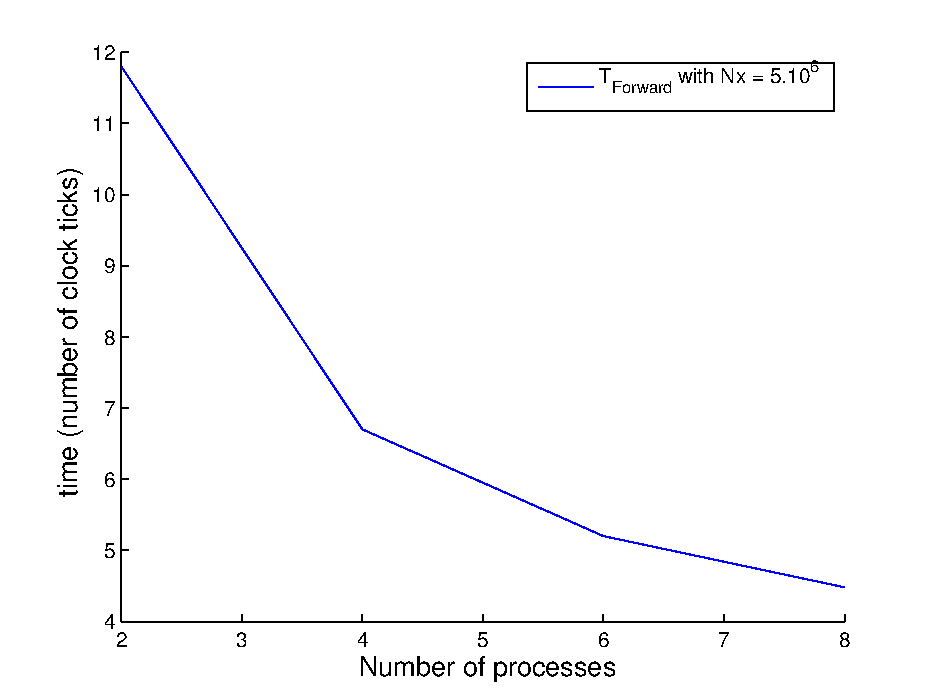
\includegraphics[width=0.8\textwidth]{figure/Forward_CB2.pdf}
\end{figure}



\hypertarget{seq-par-roukf}{}\subsection{'ReducedOrderUnscentedKalmanFilter'}\label{seq-par-roukf}


\hypertarget{seq-par-rouk-algof}{}\paragraph{Algorithm}\label{seq-par-roukf-algo}

Sampling:\\
  $ x_{h}^{(i)a} = x_h^a + L_h\sqrt{U_h^{-1}}I^{(i)} \textrm{, } \quad 1\leq i \leq p+1 $\\
  Prediction:\\
  $ x_{h+1}^f = E_\alpha(\mathcal{M}_{h}(x_{h+1}^{(*)a})) $\\
  $ x_{h+1}^{(i)f} = \mathcal{M}_{h}(x_{h}^{(i)a})$\\
  $ L_{h+1} = [x_{h+1}^{(*)f}]D_\alpha [V^*]^T \in \mathcal{M}_{n,p} $\\

  Update:\\
  $ y_{h+1}^{(i)} = \mathcal{H}_{h+1}(x_{h+1}^{(i)f})$\\
  $ \{HL\}_{h+1} = [y_{h+1}^{*}]D_\alpha [V^*]^T$\\
  $ U_{h+1} = P_{\alpha}^V +  \{HL\}_{h+1}^T R_{h+1}^{-1} \{HL\}_{h+1} \in \mathcal{M}_{p}$\\
  $ x_{h+1}^a = x_{h+1}^f + L_{h+1}U_{h+1}^{-1}\{HL\}_{h+1}^T R_{h+1}^{-1} (y_{h+1}-E_\alpha(y_{h+1}^{(*)}))$\\




\hypertarget{seq-par-roukf-ds}{}\paragraph{Distributed Structure in 'ReducedOrderUnscentedKalmanFilter'}\label{seq-par-roukf-ds}


The goal is that no variable of the model state size is allocated by any process. The concerned variables are  $x^a$, $L \in \mathcal{M}_{N_{state}, N_{sigma\_point}}$ and $ [x^{(*)f}] \in \mathcal{M}_{N_{state}, N_{reduced}}$.


\begin{itemize}

\item The state vector is a distributed dense vector whose management is delegated to the model (see Section \ref{seq-par-dm-sv}). The model state access are performed thanks to Model$::$GetState and Model$::$StateUpdated methods.

\item The sensitivity matrix $L$ is a row distributed dense matrix whose management is delegated to the model. The model is responsible for defining a a row distribution compatible with the one of the state vector (see Section \ref{seq-par-dm-cm}). The $L$ access is performed using Model$::$GetStateErrorVarianceProjector method.

\item The matrix $ [x^{(*)f}]$ must be defined as a distributed dense matrix which distribution is compatible with the one of the matrix $L$. Since the matrix  $ [x^{(*)f}]$ is peculiar to the ROUKF algorithm, its management can't be delegated to the model. Thus, it is necessary to allocate this matrix in the data assimilation method. $ [x^{(*)f}]$ construction requires two information: the type of the matrix (dense distributed) and the distribution over the processes ($[x^{(*)f}]$ distribution compatible with $L$ distribution).


$ [x^{(*)f}]$ construction must be modular: ROUKF implementation must be the same in sequential and in parallel.


\par \textcolor{red}{Specification of $ [x^{(*)f}]$ type}\\

In PETSc, the types of the structures are managed dynamically. Every matrix has the same static type 'Mat', the real type of the matrix is defined during the execution by the following function call:

\begin{frame_cpp}
Mat A;
MatSetType(A, MATMPIDENSE);
\end{frame_cpp}


Indeed, PETSc is written in C language, thus template function can't be defined for linear algebra operations. In Seldon the type of the matrices and vectors are statics. The type of $[x^{(*)f}]$ is the same as the one of $L$. It is no longer required to call any function to specify the type. (The management of the types in Verdandi is detailed in Section \ref{seq-par-type})

\par \textcolor{red}{Distribution of $ [x^{(*)f}]$}\\

The distribution of  $ [x^{(*)f}]$ is performed during the allocation. The distribution of $L$ must be provided to the constructor of matrix $[x^{(*)f}]$.



Allocation of a sequential matrix of  $\mathcal{M}_{m, n}$ :
\begin{frame_cpp}
Matrix<double> A;
A.Reallocate(m, n);
\end{frame_cpp}
Allocation of a parallel matrix of  $\mathcal{M}_{m, n}$  with a distribution of $mlocal$ rows on the local process:
\begin{frame_cpp}
Matrix<double> A;
A.Reallocate(m, n, mlocal);
\end{frame_cpp}

In order to have the same code in sequential and in parallel, the following template function is defined:
\begin{frame_cpp}
template <class Model, class T, class Prop, class Storage, class Allocator>
void Allocate(const Model& model, Matrix<T, Prop, Storage, Allocator>& A, int n, int m)
{
	A.Reallocate(m, n);
}
\end{frame_cpp}

This template function is overloaded for distributed dense matrices:
\begin{frame_cpp}
template <class Model, class T, class Prop, class Allocator>
void Allocate(const Model& model, Matrix<T, Prop, PETScMPIDense, Allocator>& A, int n, int m)
{
	A.Reallocate(m, n, model.GetLocalM());
}
\end{frame_cpp}


The allocation of  $ [x^{(*)f}]$ is perfumed in ROUKF by the following call:
\begin{frame_cpp}
Allocate(model_, X_i, Nstate, Nsigma_point);
\end{frame_cpp}

So, the implementation of ROUKF is the same in sequential and in parallel. In sequential, this implementation does not required the addition of any methods to the model interface. In parallel, the model should defined the method Model$::$GetLocalM()
which provides the number of local rows in the $L$ distribution.

\end{itemize}


\hypertarget{seq-par-roukf-p}{}\paragraph{Performance}\label{seq-par-roukf-p}

The proposed implementation enables to apply the ROUKF algorithm to a distributed model.  No variable of the model state size is allocated by any process. Thus the memory complexity is divided by the number of processes used.

Concerning the time performance, during the prediction step:

\begin{itemize}
 \item the computation  $ x_{h+1}^{(i)f} = \mathcal{M}_{h}(x_{h}^{(i)a})$ has the same speed up as the one of the model.
 \item the computation  $ L_{h+1} = [x_{h+1}^{(*)f}]D_\alpha [V^*]^T $ has a speed up equal to the number of processes.
 \end{itemize}
During the update step :
\begin{itemize}
\item the computation  $ x_{h+1}^a = x_{h+1}^f + L_{h+1}U_{h+1}^{-1}\{HL\}_{h+1}^T R_{h+1}^{-1} (y_{h+1}-E_\alpha(y_{h+1}^{(*)})) $ has a speed up equal to the number of processes.\\
\end{itemize}

The performances of the ROUKF algorithm are introduced in Figure  \ref{fig:roukf_time}.


\begin{figure}
  \caption{Simulation time of the sequential  ROUKF applied to the 'PetscClampedBar' model with $N_{state} = 5.10^6$}
  \label{fig:roukf_time}

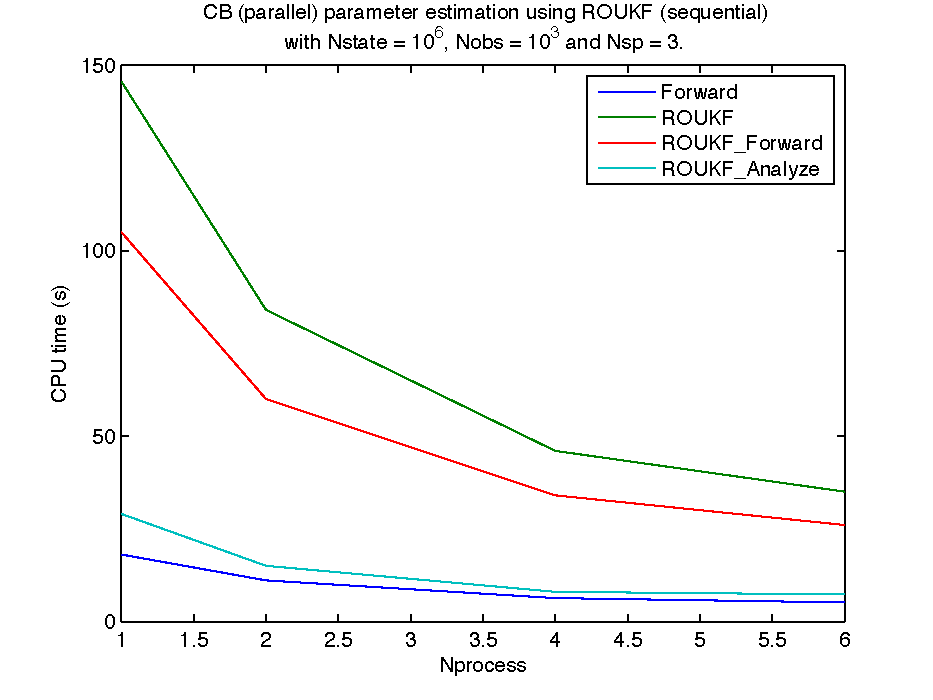
\includegraphics[width=0.8\textwidth]{figure/ROUKF_Seq_CB_Par_2.pdf}
\end{figure}



\hypertarget{seq-par-ep}{}\subsection{Example Programs}\label{seq-par-ep}

The example programs are located in the  verdandi/example/petsc\_clamped\_bar directory.


\hypertarget{seq-par-ep-c}{}\paragraph{Compilation}\label{seq-par-ep-c}


\par \textcolor{red}{Dependencies}\\


\textbf{OpenMPI}\\

\begin{itemize}

\item Download the following archive:\\
\href{http://www.open-mpi.org/software/ompi/v1.6/}{http://www.open-mpi.org/software/ompi/v1.6/}.

\item  Extract the archive and execute the following command in the source directory:

\begin{frame_bash}
$ ./configure   \
     CC=/usr/bin/gcc-4.2 \
     CPP=/usr/bin/cpp-4.2 \
     CXX=/usr/bin/g++-4.2 \
     F77=/usr/bin/gfortran \
     FC=/usr/bin/gfortran \
     F90=/usr/bin/gfortran \
     CFLAGS=-m64 \
     CXXFLAGS=-m64 \
     FFLAGS=-m64 \
     FCFLAGS=-m64 \
     LDFLAGS=-m64 \
\end{frame_bash}

\end{itemize}


\textbf{PETSc-3.3}\\

\begin{itemize}

\item Download the following archive:\\
\href{http://www.mcs.anl.gov/petsc/download/index.html}{http://www.mcs.anl.gov/petsc/download/index.html}.

\item  Extract the archive and execute the following command in the source directory:

\begin{frame_bash}
$ export PETSC_DIR=/Users/Shared/Library/Petsc
$ export PETSC_ARCH=macosx-10.7-debug
$ python config/configure.py  CXXFLAGS=-m64   CFLAGS=-m64  FCFLAGS=-m64  FFLAGS=-m64  LDFLAGS=-m64  --with-debugging=yes  --with-dynamic-loading  --with-shared-libraries  --with-parmetis-include=/Users/Shared/Library/ParMetis  --with-parmetis-lib="-L/Users/Shared/Library/ParMetis -lparmetis -lmetis" --with-metis-include=/Users/Shared/Library/Metis/64/Lib  --with-metis-lib="-L/Users/Shared/Library/Metis/64 -lmetis"  --with-superlu_dist-lib="-L/Users/Shared/Library/SuperLUDIST/lib -lsuperlu_dist"  --with-superlu_dist-include=/Users/Shared/Library/SuperLUDIST/SRC  --with-scalapack-lib="-L/Users/Shared/Library/SCALAPACK -lscalapack"  --with-scalapack-include=/Users/Shared/Library/SCALAPACK/SRC  --with-blacs-lib="-L/Users/Shared/Library/BLACS/LIB -lblacs -lblacsCinit -lblacsF77init"  --with-blacs-include=/Users/Shared/Library/BLACS/SRC  --with-mumps-include=/Users/Shared/Library/Mumps/include/ --with-mumps-lib="-L/Users/Shared/Library/Mumps/lib/ -ldmumps -lzmumps -lmumps_common -lpord -lgfortran" --with-mpi-dir=/Users/Shared/Library/OpenMPI
\end{frame_bash}

\end{itemize}


\par \textcolor{red}{Example Programs}\\


Compile the program \textbf{generate\_observation.cpp}:

\begin{frame_bash}
$ scons generate_observation mpi=yes
\end{frame_bash}

Then compile the program \textbf{reduced\_order\_unscented\_kalman\_filter.cpp}:
\begin{frame_bash}
$ scons reduced_order_unscented_kalman_filter mpi=yes
\end{frame_bash}



\hypertarget{seq-par-ep-o}{}\paragraph{Observation}\label{seq-par-ep-o}


Since no observations are given yet, we have to generate some. Execute the following command:

\begin{frame_bash}
$ mpirun -n 2 generate_observation configuration/truth.lua
\end{frame_bash}

to run the model with the initial conditions described in truth.lua, without data assimilation. This should generate a result file  \textbf{truth-state\_forecast.bin}  in the directory \textbf{example/result}. This file store the state (displacement, velocity, $\theta_f$) trajectory.
The generated state (displacement, velocity, $\theta_f$) will serve as observations for the assimilation.



\hypertarget{seq-par-ep}{}\paragraph{Data Assimilation with 'ReducedOrderUnscentedKalmanFilter'}\label{seq-par-ep}


To use the ROUKF method, execute the following command:

\begin{frame_bash}
$ mpirun -n 4 reduced_order_unscented_kalman_filter configuration/assimilation.lua
\end{frame_bash}

All processes are assigned to the model. The results should be the same as those obtained in sequential.

\hypertarget{par-par}{}\section{Parallel Method applied to Parallel Model}\label{par-par}


\hypertarget{par-par-pr}{}\subsection{Parallel 'ReducedOrderUnscentedKalmanFilter'}\label{par-par-pr}


\hypertarget{par-par-pr-mc}{}\paragraph{MPI Communicator}\label{par-par-pr-mc}


The objective is to apply the parallel ROUKF algorithm introduced in Section \ref{par-seq} on  a distributed model. We want to implement the capabilities in Verdandi to instantiate several models in parallel, and to assign several processes to each model task. A possible solution consist in using the grid topology provided by MPI:


\begin{itemize}

\item each process is defined in a MPI processor grid.

\item each process is identified by its coordinates in the grid. Figure \ref{fig:mpi_grid} represents an example of a mapping table of process rank and their corresponding grid coordinates.

\item  for each row of the grid,  a communicator containing the subgrid that includes the processes of the row is created. For instance,  in Figure \ref{fig:mpi_grid}, the group of the second row communicator is composed of processes 4, 5, 6 and 7 from $MPI\_COMM\_WORLD$ . Process 0 in second row communicator is the same as process 4 in $MPI\_COMM\_WORLD$, process 1 the same as process 5...

\item for each column of the grid,  a communicator containing the subgrid that includes the processes of the column is created.

\end{itemize}

\begin{figure}
  \caption{$4*4$ MPI Processor Grid }
  \label{fig:mpi_grid}
  \centering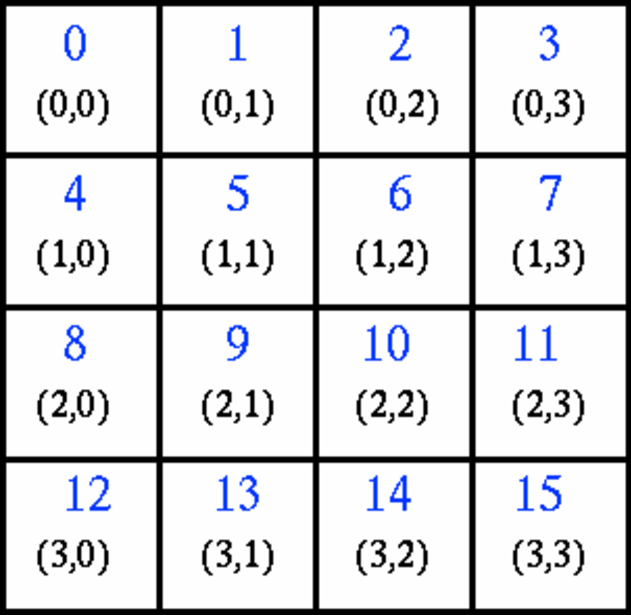
\includegraphics[width=0.4\textwidth]{figure/grid.pdf}

\end{figure}



Each column communicator correspond to an instance of model. In Figure \ref{fig:mpi_grid}, there is 4 instance of model. The first column communicator, composed of processes 0, 4, 8 and 12, is assigned to the first model instance. Then, the second column communicator is assigned to the second model instance...

Some changes  about the configuration of MPI communicators in the distributed model may be required. Indeed, the distributed model are not allowed to performed computations in the global MPI communicator $MPI\_COMM\_WORLD$. To enable several parallel model instances, $MPI\_COMM\_WORLD$ has to be replaced by a communicator of disjoint process sets in which each of the model instance operates. The column communicators to be assigned to the model instances are generated by the data assimilation method. These communicators are assigned to the model instances thanks to the following method:

\begin{frame_cpp}
namespace Verdandi
{


    //! This class is a model template.
    class ModelTemplate: public VerdandiBase
    {
        public:
            ...
            // Parallel model.
#ifdef VERDANDI_WITH_MPI
            void SetMPICommunicator(MPI_Comm& mpi_communicator);
#endif
            ...
    }

}
\end{frame_cpp}

The row communicators enable the parallel ROUKF algorithm to update its distributed variables $x^a$, $L \in \mathcal{M}_{n,p}$ and $ [x^{(*)f}] \in \mathcal{M}_{n,r}$.


\hypertarget{par-par-pr-a}{}\paragraph{Algorithm}\label{par-par-pr-a}

This Section describes the parallel ROUKF algorithm applied to a parallel model. The processes are mapped to a process grid by using row-major order (see Section \ref{par-par-pr-mc}).


\par \textbf{Initialization}

  \begin{itemize}

 \item First column  of the MPI grid (processes 0, 4, 8, 12; instance of model 0) allocates matrix $L$.\\

 \end{itemize}

 \par  \textbf{Sampling}


 \begin{itemize}

  \item First column  of the MPI grid computes  $ x_{h}^{(i)a} = x_h^a + L_h\sqrt{U_h^{-1}}I^{(i)} \textrm{, } \quad 1\leq i \leq p+1 $.

  \item First column  of the MPI grid distributes particles  $ x_{h}^{(i)a} $ over all columns.\\

 \end{itemize}

  \par  \textbf{Prediction}

   \begin{itemize}

  \item Each column  of the MPI grid computes in parallel  $ x_{h+1}^{(i)f} = \mathcal{M}_{h}(x_{h}^{(i)a})$ with its local particles.

  \item Each column of the MPI grid sends its local particles  $ x_{h+1}^{(i)f}$ to the first column.

   \item Each column of the MPI grid  computes in parallel  $ y_{h+1}^{(i)} = \mathcal{H}_{h+1}(x_{h+1}^{(i)f})$.

    \item Each column of the MPI grid sends its local particles   $ y_{h+1}^{(i)} = \mathcal{H}_{h+1}(x_{h+1}^{(i)f})$ to the first column.

  \item First column  of the MPI grid computes  $ L_{h+1} = [x_{h+1}^{(*)f}]D_\alpha [V^*]^T $.


 \end{itemize}

 \par  \textbf{Update}\\

 \begin{itemize}

 \item First column  of the MPI grid computes $ \{HL\}_{h+1} = [y_{h+1}^{*}]D_\alpha [V^*]^T$.

 \item  First column  of the MPI grid computes  $ U_{h+1} = P_{\alpha}^V +  \{HL\}_{h+1}^T R_{h+1}^{-1} \{HL\}_{h+1}$.

  \item First column  of the MPI grid computes $ x_{h+1}^a = x_{h+1}^f + L_{h+1}U_{h+1}^{-1}\{HL\}_{h+1}^T R_{h+1}^{-1} (y_{h+1}-E_\alpha(y_{h+1}^{(*)}))$.\\

 \end{itemize}



\hypertarget{par-par-ep}{}\subsection{Example Programs}\label{par-par-ep}


The example programs are located in the  verdandi/example/petsc\_clamped\_bar directory.


\hypertarget{par-par-ep-c}{}\paragraph{Compilation}\label{par-par-ep-c}


First of all, the preprocessor variable $ VERDANDI\_WITH\_MPI $ has to be defined in files  \textbf{reduced\_order\_extended\_kalman\_filter.cpp} and \textbf{reduced\_order\_unscented\_kalman\_filter.cpp}:

\begin{frame_cpp}
#define VERDANDI_DEBUG_LEVEL_4
#define SELDON_WITH_BLAS
#define SELDON_WITH_LAPACK

#define VERDANDI_WITH_ABORT
#define VERDANDI_DENSE

#define VERDANDI_WITH_MPI

#if defined(VERDANDI_WITH_MPI)
#include <mpi.h>
#endif


#include "Verdandi.hxx"
#include "seldon/SeldonSolver.hxx"

#include "model/PetscClampedBar.cxx"
#include "observation_manager/PetscLinearObservationManager.cxx"
#include "method/ReducedOrderUnscentedKalmanFilter.cxx"


int main(int argc, char** argv)
{

    VERDANDI_TRY;

    ...
}
\end{frame_cpp}

Compile the program \textbf{generate\_observation.cpp}:

\begin{frame_bash}
$ scons generate_observation mpi=yes
\end{frame_bash}

Then compile the program \textbf{reduced\_order\_unscented\_kalman\_filter.cpp}:
\begin{frame_bash}
$ scons reduced_order_unscented_kalman_filter mpi=yes
\end{frame_bash}



\hypertarget{par-par-ep-o}{}\paragraph{Observation}\label{par-par-ep-o}


Since no observations are given yet, we have to generate some. Execute the following command:

\begin{frame_bash}
$ mpirun -n 2 generate_observation configuration/truth.lua
\end{frame_bash}

to run the model with the initial conditions described in truth.lua, without data assimilation. This should generate a result file  \textbf{truth-state\_forecast.bin}  in the directory \textbf{example/result}. This file store the state (displacement, velocity, $\theta_f$) trajectory.
The generated state (displacement, velocity, $\theta_f$) will serve as observations for the assimilation.


\hypertarget{par-par-ep}{}\paragraph{Data Assimilation with 'ReducedOrderUnscentedKalmanFilter'}\label{par-par-ep}


The parameters of the ROUKF method are described in the configuration file  \textbf{configuration/assimilation.lua}.

It is necessary to define the dimension of the MPI grid. The number of model instances and the number of processes assigned to each model instance must be defined:

\textbf{assimilation.lua}\\
\begin{frame_lua}
-- Simulation with assimilation using ROUKF.
reduced_order_unscented_kalman_filter = {

 	...

   mpi_grid = {

      -- The number of processes for each model task.
      Nrow = 2,
      -- The number of model tasks.
      Ncol = 3
   }

}

\end{frame_lua}

To use the ROUKF method, execute the following command:

\begin{frame_bash}
$ mpirun -n 6 reduced_order_unscented_kalman_filter configuration/assimilation.lua
\end{frame_bash}

\textbf{Warning:} The number of processes must be equal to $mpi\_grid.Nrow * mpi\_grid.Nco$.


The results should be the same as those obtained in sequential.

\hypertarget{par-par-p}{}\section{Performance}\label{par-par-p}


\begin{figure}
  \caption{PetscClampedBar parameter estimation using ROUKF (parallel) with $N_{state} = 10^5$ and $N_{observation} = 10^4$ }

  \vspace{1cm}

  \label{fig:roukf_par_time}
  \centering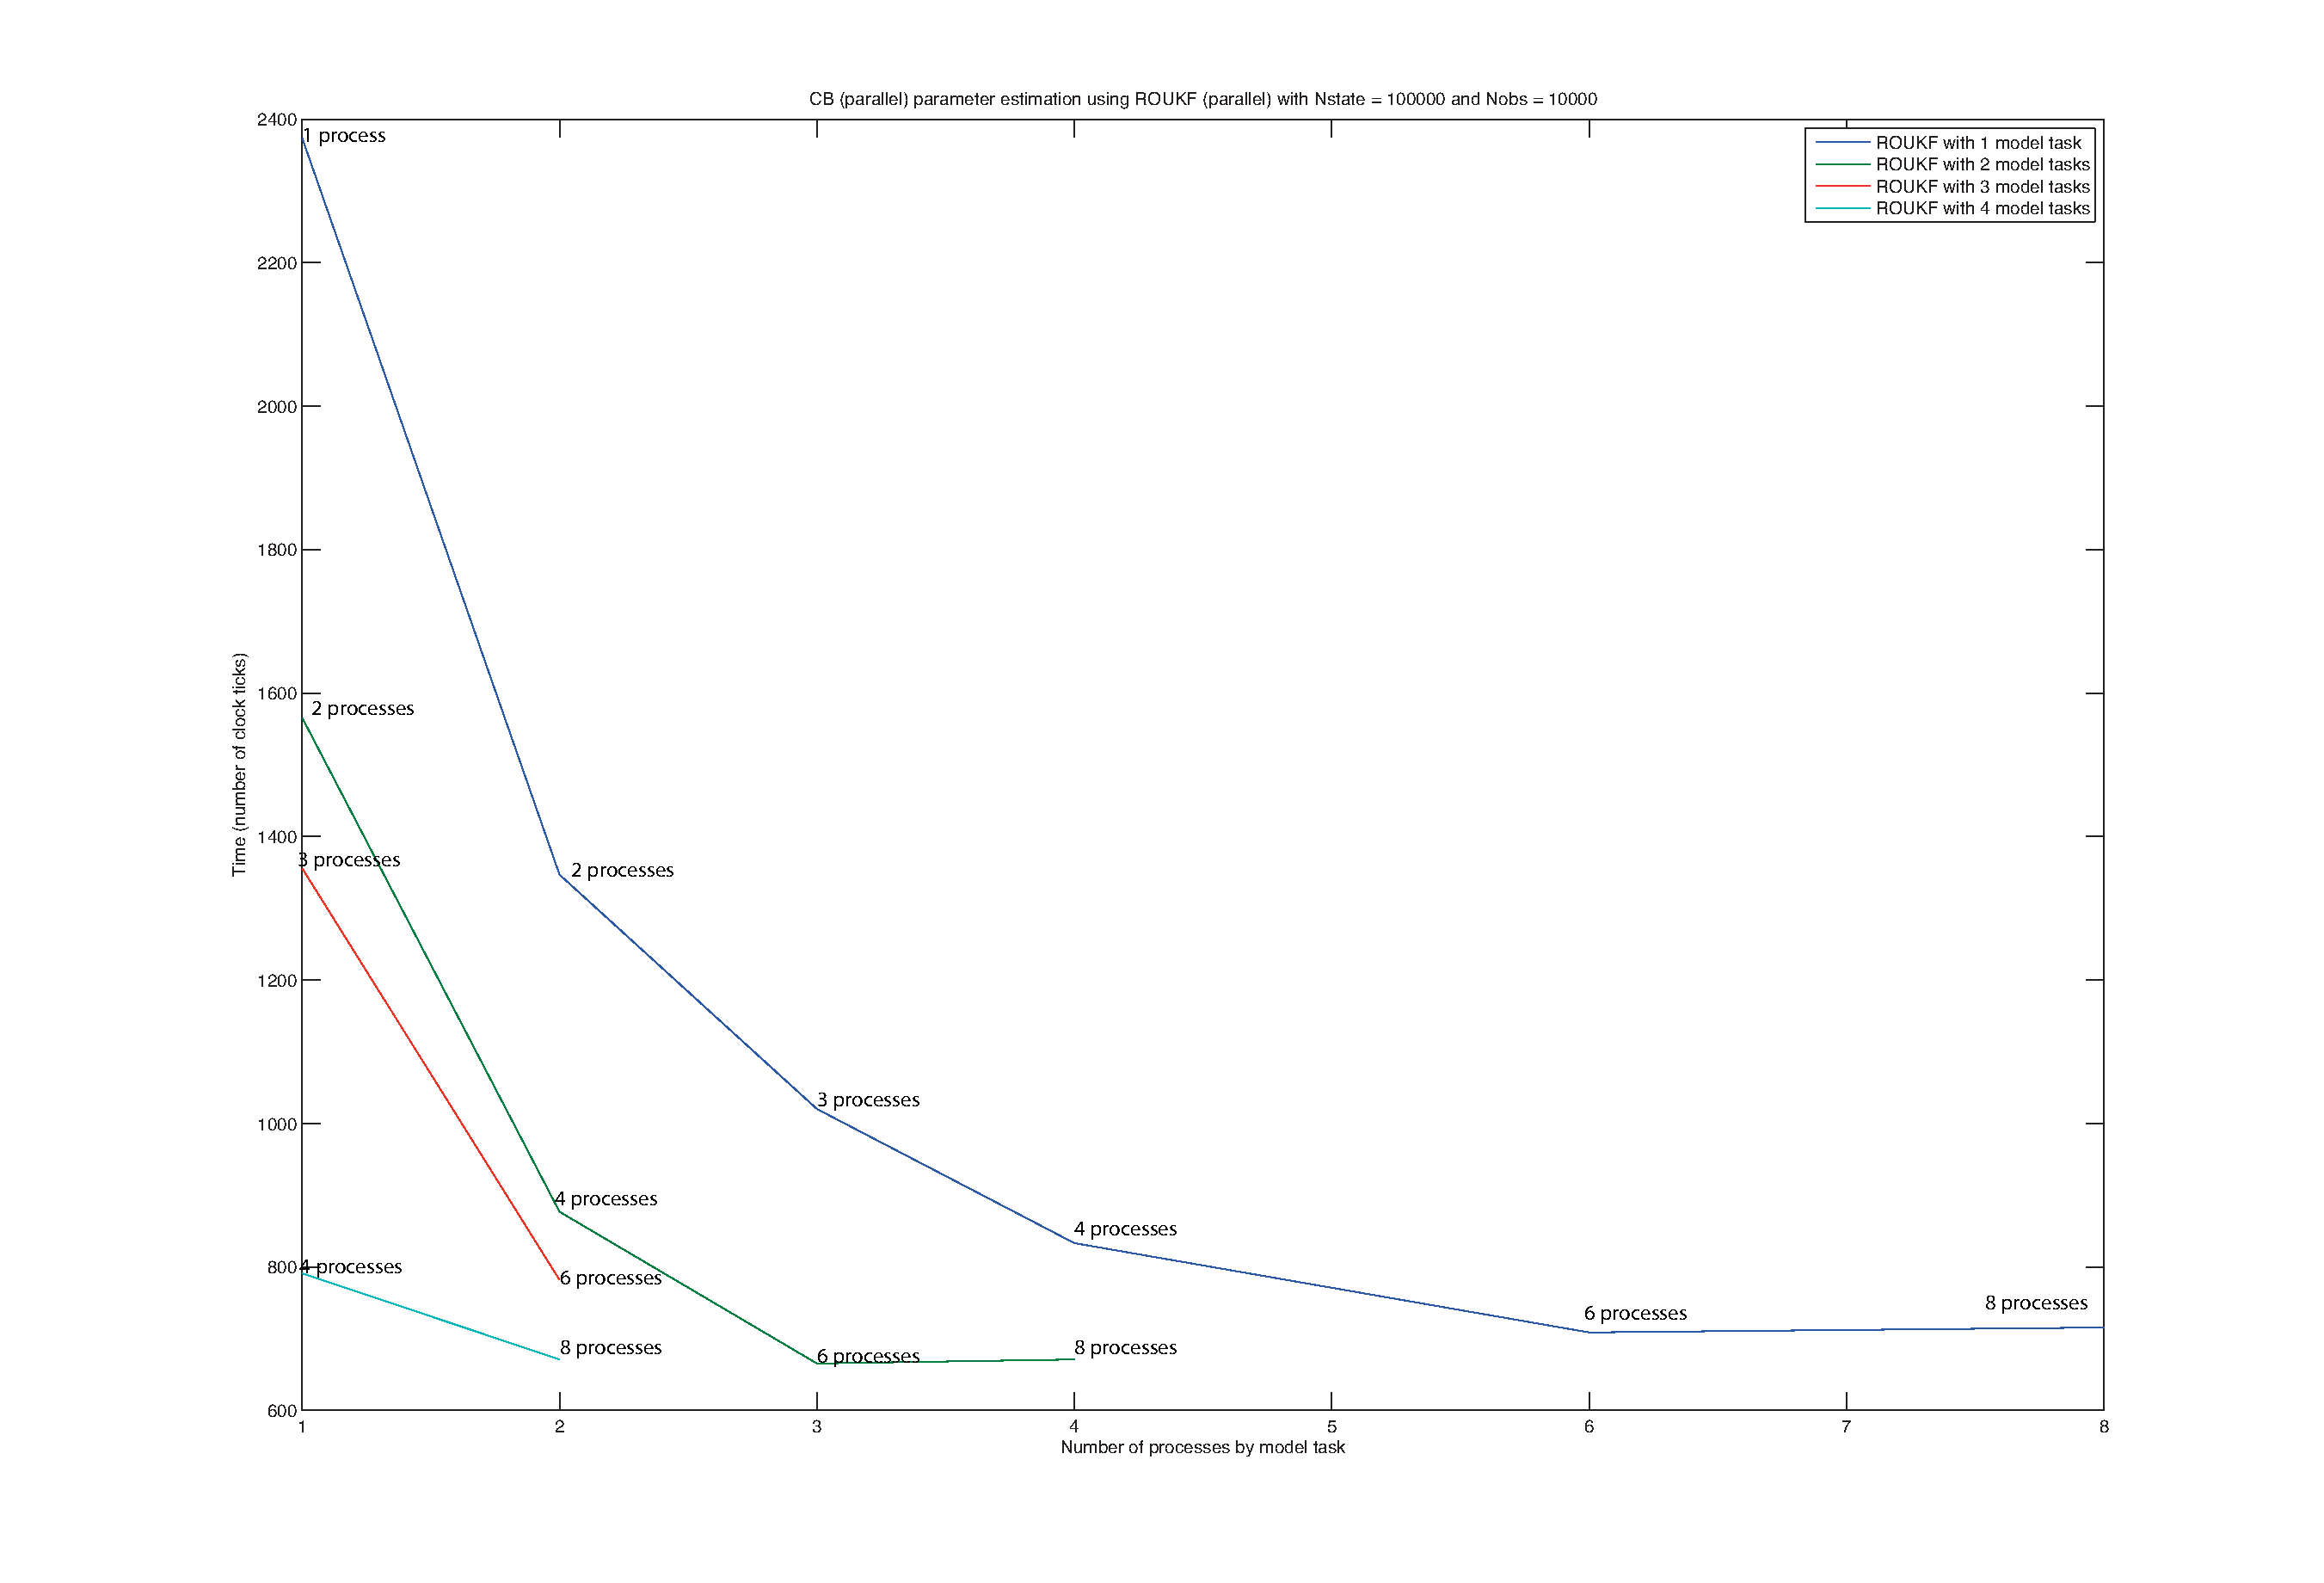
\includegraphics[width=1.\textwidth]{figure/roukf_par_3_test.pdf}
\end{figure}


We can see in Figure \ref{fig:roukf_par_time} that when the number of processes is less than or equal to four, it is more in efficient to instantiate only one model and to assign all processes to this instance. On the other hand, when the number of processes increases, the most effective is to own
several model instances:

\begin{itemize}

\item when the number of processes is equal to sox, the most efficient is to define two model instances running on three processes.

\item when the number of processes is equal to sox, the optimal configuration is to have two model instances running on four processes.

\end{itemize}


As intended, this second level of parallelism provides a better scalability. At the fist level of parallelism, when the efficiency of ROUKF algorithm decreases, this second level of parallelism contributes to better take advantage of the  available computation resources.

\part{Example Models}
\chapter{Example Models}
\label{example_models}
\hypertarget{example_models}{}
\input{example_models}
\chapter{Clamped Bar}
\label{clamped_bar_model}
\hypertarget{clamped_bar_model}{}
\input{clamped_bar_model}
\chapter{Lorenz model}
\label{lorenz_model}
\hypertarget{lorenz_model}{}
\input{lorenz_model}
\chapter{Quadratic Model}
\label{quadratic_model}
\hypertarget{quadratic_model}{}
\input{quadratic_model}
\chapter{Shallow-\/water}
\label{shallow_water_model}
\hypertarget{shallow_water_model}{}
\input{shallow_water_model}
\part{Example Observation Managers}
\chapter{Observations}
\label{observations}
\hypertarget{observations}{}
\input{observations}
\chapter{Grid To Network Observation Manager}
\label{grid_to_network_observation_manager}
\hypertarget{grid_to_network_observation_manager}{}
\input{grid_to_network_observation_manager}
\chapter{Linear Observation Manager}
\label{linear_observation_manager}
\hypertarget{linear_observation_manager}{}
\input{linear_observation_manager}
\chapter{Observation Aggregator}
\label{observation_aggregator}
\hypertarget{observation_aggregator}{}
\input{observation_aggregator}
\part{Plugging in Verdandi}
\chapter{Plugging in Verdandi}
\label{plugging_in_verdandi}
\hypertarget{plugging_in_verdandi}{}
\input{plugging_in_verdandi}
\chapter{Plugging a Model}
\label{plugging_model}
\hypertarget{plugging_model}{}
\input{plugging_model}
\chapter{Plugging a Python model}
\label{plugging_python_model}
\hypertarget{plugging_python_model}{}
\input{plugging_python_model}
\chapter{Methods requirements for models}
\label{model_requirements}
\hypertarget{model_requirements}{}
\input{model_requirements}
\chapter{Methods requirements for observation managers}
\label{observation_requirements}
\hypertarget{observation_requirements}{}
\input{observation_requirements}
\chapter{Plugging the Observation Manager}
\label{plugging_observation}
\hypertarget{plugging_observation}{}
\input{plugging_observation}
\part{Tools}
\chapter{Tools}
\label{tools}
\hypertarget{tools}{}
\input{tools}
\chapter{Perturbation manager}
\label{perturbation_manager}
\hypertarget{perturbation_manager}{}
\input{perturbation_manager}
\chapter{Optimization Solver}
\label{optimization_solver}
\hypertarget{optimization_solver}{}
\input{optimization_solver}
\part{Developing in Verdandi}
\chapter{Dependencies}
\label{dependencies}
\hypertarget{dependencies}{}
\input{dependencies}
\chapter{Linear Algebra Library}
\label{linear_algebra}
\hypertarget{linear_algebra}{}
\input{linear_algebra}
\chapter{Coding Standard}
% Copyright (C) 2009, INRIA
% Author(s): Vivien Mallet
%
% You can redistribute this document and/or modify it under the terms of the
% GNU General Public License as published by the Free Software Foundation;
% either version 2 of the License, or (at your option) any later version.
%
% This document is distributed in the hope that it will be useful, but WITHOUT
% ANY WARRANTY; without even the implied warranty of MERCHANTABILITY or
% FITNESS FOR A PARTICULAR PURPOSE. See the GNU General Public License for
% more details.

\newcounter{points}

\newcommand{\cscode}[1]{\texttt{#1}}
\newcommand{\csrule}[1]{\textsc{#1}}
\newcommand{\cscomment}[1]{\newline #1}
\newcommand{\cscommentf}[1]{#1}
\newcommand{\csjustification}[1]{\newline {\it Justification} --- #1}
\newcommand{\csnjustification}[1]{{\it Justification} --- #1}
\newcommand{\csjustificationf}[1]{#1}

\newenvironment{cenumerate}
{
  \begin{enumerate}\setcounter{enumi}{\value{points}}%
  }
  {
    \setcounter{points}{\value{enumi}}\end{enumerate}
}

%%%%%%%%%%%%%%%%%%
%% INTRODUCTION %%
%%%%%%%%%%%%%%%%%%


\section*{Introduction}
\label{part:introduction}

Many coding standards may be found on-line: see, for instance, the list
provided at \url{http://www.chris-lott.org/resources/cstyle/}. In particular,
the \textit{C++ Coding Standard} by Todd Hoff, available at
\url{http://www.possibility.com/Cpp/CppCodingStandard.html} provided useful
guidelines for the present standard.

The general conventions of part~\ref{part:general} shall be applied to all
computer codes, in any language. C++ conventions follow in
part~\ref{part:cpp}.


%%%%%%%%%%%%%%%%%%%
%% GENERAL RULES %%
%%%%%%%%%%%%%%%%%%%


\section{General Conventions}
\label{part:general}

The following conventions must be applied in all languages.

\subsection{Development}

\begin{enumerate}
\item \csrule{Codes must be written in American English. This includes variable
    names, file names, comments,~\ldots{}} \csjustification{A code should be
    open to anyone.  Even if a code is not intended to be shared initially,
    this may change.  Moreover parts of it may be reused in another project.}
\item \csrule{Optimize only the parts of the code that lead to significant
    overheads.} \cscomment{In addition, remember that the compilers partially
    optimize your code.} \csjustification{An optimized code is usually less
    readable than its straightforward version.}
\item \csrule{A code must compile without warnings.}  \cscomment{At development
    stage, compile your code with the most restrictive compilation options and
    with all warning messages enabled.} \csjustification{It increases
    portability, and it may help avoiding mistakes.}
\item \csrule{Global variables must be avoided.} \csjustification{Units of a code
    should be independent from their environment so that they may be reused
    and so that the overall code may be safer.}
  \setcounter{points}{\value{enumi}}
\end{enumerate}


\subsection{Names}

\begin{cenumerate}
\item \csrule{Use explicit and meaningful names.} \cscomment{You should first
    consider that the length does not matter. Actually it does, but many
    programmers tend to use too short and therefore uninformative
    names. Usually, the wider scope, the longer name.}  \csjustification{New
    programmers should be able to read the code without learning the meaning
    of the variables and the functions in use. Explicit names also save
    unnecessary comments.  Example (in C++):}
\begin{verbatim}
if (Species.GetName() == target_species)
    output_concentration = Species.Concentration();
\end{verbatim}
  \csjustificationf{is better than:}
\begin{verbatim}
// Checks whether current species is the target species.
if (sp.GetName() == species)
    // Retrieves the output concentration.
    c = sp.Concentration();
\end{verbatim}
\item \csrule{Avoid contractions. If you really need a contraction, only use it
    as a suffix.} \cscomment{Accepted contractions are: tmp (temporary), in
    (input), out (output), obs (observation). Example: \cscode{value\_in}.}
  \csjustification{Contractions can easily collide (including with a full word)
    or have meanings depending on the context. Besides, not all developers may
    understand your contractions, depending on their habits and maybe their
    native language. For instance, French developers often contract
    \cscode{number} into \cscode{nb} whereas a native English speaker would use
    \cscode{num}.}
\item \csrule{Unless a more explicit name is found, preferably use {\rm
      \cscode{i}} for an index. As for dimensions, use {\rm \cscode{h}} for time
    index, {\rm \cscode{i}} along x, {\rm \cscode{j}} along y and {\rm \cscode{k}}
    along z.} \csjustification{This is a common practice.}
\item \csrule{Avoid plural forms.} \cscomment{Even the name of a vector should not
    be in plural form. For instance, a vector of observations can be called
    \cscode{observation}, and the i-th observation is \cscode{observation(i)}
    which is perfectly clear. If the plural form seems to be required,
    consider appending \cscode{\_list}: e.g., \cscode{location =
      location\_list(i)}, even if \cscode{location\_list} is not an instance of
    the STL class \cscode{list}.} \csjustification{The use of plural forms makes
    it difficult to guess or remember the names of variables and methods. It
    is quickly unclear whether the plural form was used or not for such and
    such methods. The same is true with a complex object that stores many data
    sets: should it be named with plural form because it contains a list, or
    should the singular be preferred because it appears as a single
    block/object? The easiest way to avoid the confusion is to avoid plural
    forms.}
\item \csrule{A fixed number of \cscode{xxx} should be named \cscode{Nxxx}.}
  \cscomment{Example: \cscode{Nstep} for the number of steps (if it is fixed),
    \cscode{Narray} for a number of arrays.}
\item \csrule{The Boolean methods should have a prefix like \cscode{Is} or
    \cscode{Has}.} \cscomment{Examples: \cscode{IsReady}, \cscode{HasObservation},
    \cscode{IsEmpty}.} \csjustification{It makes it clear that the method returns
    a Boolean. The question that the method answers is very clear too.}
\end{cenumerate}


\subsection{Formatting}

\subsubsection{Spaces and Parens}
\label{sec:spaces-parens}

\begin{cenumerate}
\item \csrule{Put one blank space before and one blank space after the
    operators: \cscode{+}, \cscode{-}, \cscode{/}, \cscode{*} (multiplication),
    \cscode{=}, \cscode{+=}, \cscode{-=}, \cscode{*=}, \cscode{/=}, \cscode{|}, \cscode{\&},
    \cscode{||}, \cscode{\&\&}, \cscode{<}, \cscode{<=}, \cscode{>}, \cscode{>=},
    \cscode{==}, \cscode{!=}, \cscode{<{}<}.}  \cscomment{You might break this rule in
    inner parens (at a deep level, e.g., some array index like \cscode{i+1} in a
    complex formula).} \csjustification{It makes the code much more readable. It
    is also a very common practice.}
\item \csrule{Put one blank space after each comma.} \csjustification{It makes the
    code more readable. It is a very common practice.}
\item \csrule{Do not add trailing spaces at the end of code lines.} \cscomment{A
    script can remove the trailing spaces for you---such a script should be
    run before any commit to the repository of your revision control
    system. Emacs users may have their editor removing the trailing spaces
    whenever they save a file. They can also have Emacs show them the trailing
    whitespaces; e.g., in Python mode:}
\begin{verbatim}
(setq whitespace-style '(trailing))
(add-hook 'python-mode-hook 'whitespace-mode)
\end{verbatim}
  \csnjustification{Browsing the code, moving blocks, copies,~\ldots{} are
    slowed down because of trailing spaces. In addition, the differences
    between two revisions of a file should not include such noise.}
\item \csrule{No space between the function name and its arguments list.}
  \cscomment{Write}
\begin{verbatim}
  func(a, b)
\end{verbatim}
  \cscommentf{instead of}
\begin{verbatim}
  func (a, b)
\end{verbatim}
\item \csrule{No space after an opening paren or a closing paren.}
  \cscomment{Write}
\begin{verbatim}
  func(a, b)
\end{verbatim}
  \cscommentf{instead of}
\begin{verbatim}
  func( a, b )
\end{verbatim}
\item \csrule{Put a space between a language keyword and the following paren.}
  \cscomment{Write}
\begin{verbatim}
  while (error > epsilon)
\end{verbatim}
  \cscommentf{instead of}
\begin{verbatim}
  while(error > epsilon)
\end{verbatim}
  \csnjustification{Keywords and functions should be distinguishable.}
\item \csrule{Do not put unnecessary parens in logical expressions, except to
    clarify the order of evaluation.}  \cscomment{For instance (in C++), write}
\begin{verbatim}
  if (i != 0 && j > 5)
\end{verbatim}
\cscommentf{instead of}
\begin{verbatim}
  if ((i != 0) && (j > 5))
\end{verbatim}
\csnjustification{Unncessary parens slow down the reading.}
\end{cenumerate}

\subsubsection{Comments}

\begin{cenumerate}
\item \csrule{A comment line is placed before the lines or the block it
    comments.}  \cscomment{Observe where each comment line is placed:}
\begin{verbatim}
// Checks the availability of observations. Note that the call implicitly
// loads the observations at current date.
if (observation_manager.HasObservation())
// Assimilates the available observations.
{
    Analyze();
    if (positive_state)
        // Enforces the positivity of the state vector.
        for (int i = 0; i < Nstate; i++)
            state(i) = max(0., state(i));
}
\end{verbatim}
  \csnjustification{Since an explanation may address several lines, the scope of
    a comment placed after is unclear.}
\item \csrule{Like a sentence, a comment starts with a capital and ends with a
    dot (even a one-word comment).}  \csjustification{All comment lines should
    be consistent. This rule is clear and easy to follow.}
\item \csrule{Use simple present to explain what a line does or what a sequence
    of lines does.} \cscomment{See the example above.} \csjustification{A comment
    introduces to what a line {\it does}. So \cscode{// Extracts data.}
    implicitly means \cscode{// This line extracts data.}}
\item \csrule{When referring to a variable, surround the variable name with
    simple quotes.} \cscomment{Example: \cscode{// Updates 'state' so that it
      should be consistent with 'full\_state'.}}  \csjustification{Reading
    comments, with variable names included, can be really difficult because
    the variable names are often words: one cannot identify at first sight
    that the variable name is a special element. Think of a comment line like
    \cscode{// Makes a consistent with the location.}  instead of \cscode{// Makes
      'a' consistent with the location.}}
\end{cenumerate}

\subsubsection{Function and Method Definition}

\begin{cenumerate}
\item \csrule{Arguments are sorted from input variables to output variables.
    Dimensions are provided first.} \cscomment{The only exception is for
    optional arguments if they are necessarily the last arguments (as in C++
    and Python). Try to sort all arguments so that the order makes sense. For
    instance, if the input variables are a number of points along $x$, the
    abscissae and the values of a function $f$ at these abscissae, then
    provide them in that order. Indeed, one needs first the number of points
    $n$, then the positions $x_i$ of the points ($i\in\llbracket{}0,
    n-1\rrbracket$) and finally the associated values $f(x_i)$.}
  \csjustification{A code line is read from left to right, and obviously an
    input comes before an output.}
\end{cenumerate}


\subsection{Language Features}

\subsubsection{Standard}

\begin{cenumerate}
\item \csrule{Build a fully standard-compliant code. If a compiler does not
    understand it, discard it or maybe maintain specific code for it.}
  \csjustification{This ensures portability and makes the code perennial.}
\end{cenumerate}


%%%%%%%%%
%% C++ %%
%%%%%%%%%


\section{C++}
\label{part:cpp}


\subsection{Development}

\begin{cenumerate}
\item \csrule{Compilation with GNU G++ and with options {\rm \cscode{-Wall -ansi
        -pedantic}} should not issue any warning.} \csjustification{It increases
    portability (through compliance with the C++ standard), and it may help
    avoiding mistakes.}
\end{cenumerate}


\subsection{Names}

\subsubsection{Common Conventions}

\begin{cenumerate}
\item \csrule{Do not add a prefix to a set of objects to avoid conflicts.}
  \cscomment{Use name spaces instead.}
\end{cenumerate}

\subsubsection{Classes and Methods}

\begin{cenumerate}
\item \csrule{A name is one word or a concatenation of words. The first letter
    of each word (including the first one) is uppercase.}  \cscomment{Examples:}
\begin{verbatim}
class FormatBinary;
double Data::GetMax() const;
void Data::Print() const;
void LoadPreviousAnalysis(...);
\end{verbatim}
  \csnjustification{Two other conventions are widely used: \cscode{formatBinary}
    and \cscode{format\_binary}. With the latter convention, classes and methods
    are not easily identified in a code. The former convention is a bit
    inconsistent: one-word methods are not as emphasized as two-word methods
    are.}
\item \csrule{The accessors should be named with {\rm \cscode{Get}} or {\rm
      \cscode{Set}} (prefixed).} \cscomment{Example: \cscode{GetDate},
    \cscode{SetPosition}}.
\end{cenumerate}

\subsubsection{Functions}

\begin{cenumerate}
\item \csrule{Same rules as for the methods.} \cscomment{Meanwhile, the name of a
    small function (e.g., a single formula, or an extension of the C++
    libraries) may be lowercase with underscores to delimit the words.}
\item \csrule{Extern functions should be lowercase with underscores to delimit
    the words, and they should be prefixed by an underscore.}  \cscomment{The
    name of an extern function is defined by the compiler. If the compiler
    does comply with this convention, define a macro that follows this
    convention. Example:}
\begin{verbatim}
#define _linear_interpolation linear_interpolation_
\end{verbatim}
  \csnjustification{Fortran functions are usually named with one or two
    underscores at the end. The rule is consistent with the addition of an
    underscore, but as a prefix in order to avoid conflicts (with attributes,
    see below).}
\end{cenumerate}

\subsubsection{(Local) Variables}

This section also applies to method arguments and function arguments.

\begin{cenumerate}
\item \csrule{Use lower case and words delimited with underscores.}
  \csjustification{Many variables are naturally lowercase, like the indexes. In
    addition, one may declare an instance of a class, say \cscode{Data} or
    \cscode{ObservationManager}, with the same name as the class: \cscode{Data
      data} or \cscode{ObservationManager observation\_manager}.}
\end{cenumerate}

\subsubsection{Attributes}

\begin{cenumerate}
\item \csrule{Same rules as for variables, except that an underscore must be
    appended at the end of the name.} \cscomment{This rule might be broken in
    case the attribute is public or for consistency with a public attribute
    that has no appended underscore.} \csjustification{The underscore at the end
    enables to distinguish attributes from local variables within the
    methods. The scope is an important property of a variable. In addition,
    the method arguments may have the same names as the attributes, without
    the underscore. For example:}
\begin{verbatim}
void ExtendedStream::SetDelimiter(delimiter)
{
    delimiter_ = delimiter;
}
\end{verbatim}
\end{cenumerate}

\subsubsection{References, Pointers, Global Variables and Constant Variables}

\begin{cenumerate}
\item \csrule{No special notation is associated with references, pointers,
    global variables or constant variables.} \csjustification{Constant variables
    are declared as such (keyword \cscode{const}); no alteration of these
    variables can occur.  Global variables should be avoided. References are
    used in C++ to manipulate variables just like others: a notation to
    distinguish them would break this advantage.  Programmers sometimes prefix
    a 'p' for pointers, but the syntax is usually clear enough to show that a
    pointer is in use.}
\end{cenumerate}

\subsubsection{Name Spaces}

\begin{cenumerate}
\item \csrule{Name spaces are mainly used for libraries. A name space has the
    exact name of its library.} \cscomment{Example:}
\begin{verbatim}
namespace Verdandi;
\end{verbatim}
\end{cenumerate}

\subsubsection{Type Names (typedef)}

\begin{cenumerate}
\item \csrule{Use lower case and words delimited with underscores. Do not append
    an underscore even if the type name is defined in a class.}
  \csjustification{Type names are used as shortcuts for what may be seen as a
    low-level type, just like a \cscode{string} or a \cscode{double} in the
    \cscode{main()} function.}
\end{cenumerate}

\subsubsection{Macros}

\begin{cenumerate}
\item \csrule{Use upper case and words delimited by underscores.}
  \csjustification{Macros should be clearly identified because of their really
    specific nature. In addition, this is common practice.}
\item \csrule{In case a macro is related to a library, the first word of the
    macro must be the library name.} \cscomment{Example:}
\begin{verbatim}
  #define VERDANDI_DEBUG_LEVEL_4
\end{verbatim}
  \csnjustification{This avoids conflicts with macros from other libraries, and
    it better indicates what the macro is for.}
\end{cenumerate}


\subsection{Formatting}
\label{sec:formatting}

\subsubsection{Indentation and Braces}
\label{sec:indentation-braces}

\begin{cenumerate}
\item \csrule{Use the Allman standard for indentation.} \cscomment{This
    indentation style is called BSD under Emacs. It looks like this:}
\begin{verbatim}
    if (i == f(a, b))
        i += 5;  // No braces for a single line.
    else
    {   // Instead of "else {".
        while (i != 5)
        {
            j = 3 * f(4, b);
            i++;
        }
        i--;
    }
\end{verbatim}
  \cscommentf{Note the (compulsory) 4-space depth for the indentation. Emacs
    users can enforce this convention with the following code (placed in
    \cscode{.emacs}):}
\begin{verbatim}
(defun verdandi-c++-mode ()
  (interactive)
  (c-set-style "bsd")
  (setq c-basic-offset 4)
  (add-hook 'before-save-hook 'delete-trailing-whitespace t t))
(defun verdandi-c++-mode-hook ()
  (if (string-match "verdandi" buffer-file-name)
      (verdandi-c++-mode)))
(add-hook 'c++-mode-hook 'verdandi-c++-mode-hook)
\end{verbatim}
  \cscommentf{The hook \cscode{delete-trailing-whitespace} will remove trailing
    spaces when the file is saved, which is another formatting rule (see
    section~\ref{sec:spaces-parens}). The Verdandi C++ mode will be applied to
    any file that contains the word ``verdandi'' in its absolute path.}
  \csjustification{Consistent indentation is utterly required at least to browse
    the code and to grasp its structure. In addition, differences between two
    versions of a same code are easier to parse with a standard indentation.}
\item \csrule{Tabulations are forbidden. They should be replaced with
    spaces.}\cscomment{Emacs users can add the following line in their
    \cscode{.emacs}:}
\begin{verbatim}
(setq-default indent-tabs-mode nil)
\end{verbatim}
  \csnjustification{Tabulation-based indentation may be more convenient for code
    browsing than space-based indentation: moving in the code may be
    faster. Unfortunately, the length of a tabulation may vary from one
    environment to another (usual values are 4 or 8 spaces, maybe 2
    sometimes). This can cause misalignment. Take for example:}
\begin{verbatim}
< TAB >if (condition)
< TAB >< TAB >long_function_name(a, b, c,
< TAB >< TAB >< TAB >< TAB >....h, j, i);
\end{verbatim}
  \csjustificationf{where \cscode{< TAB >} is a tabulation and \cscode{.} is a
    whitespace. If the tabulation length is decreased, the code may look
    misaligned:}
\begin{verbatim}
<TAB>if (condition)
<TAB><TAB>long_function_name(a, b, c,
<TAB><TAB><TAB><TAB>....h, j, i);
\end{verbatim}
  \csjustificationf{where \cscode{h, j, i} is not properly placed. A clever
    solution is to use tabulations for block indentation and to use spaces for
    alignment:}
\begin{verbatim}
< TAB >if (condition)
< TAB >< TAB >long_function_name(a, b, c,
< TAB >< TAB >...................h, j, i);
\end{verbatim}
  \csjustificationf{In that configuration, the formatting will be fine whatever
    the tabulation length. Unfortunately, it seems that only Emacs and vi
    implement that formatting. In addition, the interaction between such a
    convention and the limit on the line length may be an issue. To conclude,
    the safest indentation strategy is to use spaces only, which any decent
    editor should handle:}
\begin{verbatim}
....if (condition)
........long_function_name(a, b, c,
...........................h, j, i);
\end{verbatim}
\item \csrule{The indentation depth is four spaces.} \csjustification{The
    indentation depth is usually four spaces (like in GNU coding standards) or
    eight spaces (like in Linux kernel). In scientific computing, several
    indentation levels are commonly required---for example for loops in
    three-dimensional space. A eight-space indentation depth is not practical
    in that context.}
\item \csrule{Do not put a useless semi-colon at the end of a block.}
  \cscomment{Only classes and structures declarations require a semi-colon after
    the closing brace.}
\end{cenumerate}

\subsubsection{Comments and Documentation}
\label{sec:comm-docum}

\begin{cenumerate}
\item \csrule{Use \cscode{//}, not \cscode{/*}, except for Doxygen comments.}
\item \csrule{Include Doxygen comments for every class, every attribute, every
    method and every function.}
\item \csrule{With respect to Doxygen comments of functions and methods:
    \begin{itemize}
    \item there must be a brief description, introduced by {\rm \cscode{//!}},
      or {\rm \cscode{$\backslash$*! $\backslash$brief}} if the description does
      not fit into a single line;
    \item there must be a description for every argument and for the returned
      value:
      \begin{itemize}
      \item only use {\rm \cscode{$\backslash$param[in]}}, {\rm
          \cscode{$\backslash$param[in,out]}} and {\rm
          \cscode{$\backslash${param[out]}}} to introduce the description for an
        argument;
      \item the description for an argument starts lowercase and ends with a
        dot;
      \item the description for a returned value starts with a capitalized
        word and ends with a dot.
      \end{itemize}
    \item a full description should also be added whenever necessary, just
      before the arguments description;
    \item any reference to an argument, say {\rm \cscode{x}}, should be
      introduced with the Doxygen command {\rm \cscode{$\backslash$a}}: {\rm
        \cscode{$\backslash$a x}}.
    \end{itemize}~}
    \cscomment{Template:}
\begin{verbatim}
//! Here comes the brief description.
/*! Here comes the long description, if needed.
  \param[in] x description of the first parameter. It may include several
  sentences on several lines.
  \param[in,out] value another parameter.
  \param[out] error true if and only if an error occurred.
*/
\end{verbatim}
  \cscommentf{Another template:}
\begin{verbatim}
/*! \brief Here goes a brief description that does not fit into a single
  line. */
/*! Here comes the long description, if any.
  \param[in] value description of the argument.
  \return The sign of \a value.
*/
\end{verbatim}
  \csnjustification{These rules ensure that the Doxygen documentation is
    complete and clean.}
\item \csrule{Doxygen comments for functions and methods are put before the
    definition in the source file, not before the declaration in the header
    file.} \csjustification{Headers should be as light as possible so that one
    may browse them quickly.}
\item \csrule{Doxygen comments for classes and attributes are put before their
    declarations, in the header file.} \cscomment{For attributes, the
    description is introduced by {\rm \cscode{//!}}, or {\rm
      \cscode{$\backslash$*! $\backslash$brief}} if it does not fit into a
    single line.} \csjustification{There is no other suitable place.}
\item \csrule{The code may be organized in sections and subsections that are
    introduced as follows.}  \cscomment{Section:}
\begin{verbatim}
  <two blank lines>
  ////////////////////////
  // READS INPUT FIELDS //
  ////////////////////////
  <two blank lines>
\end{verbatim}
  \cscommentf{Long section (especially in libraries, with many functions in the
    section---otherwise prefer the previous format):}
\begin{verbatim}
  <two blank lines>
  ///////////////////////////
  // MATRIX FACTORIZATIONS //
  <two blank lines>
  [ code of the long section ]
  <two blank lines>
  // MATRIX FACTORIZATIONS //
  ///////////////////////////
  <two blank lines>
\end{verbatim}
\cscommentf{Heavy subsection:}
\begin{verbatim}
  <two blank lines>
  /****************
   * Binary files *
   ****************/
  <two blank lines>
\end{verbatim}
\cscommentf{Light subsection (prefer this to the heavy subsection, except if the
  subsection is long---you may then nest light subsections inside the heavy
  subsection):}
\begin{verbatim}
  <one blank line>
  /*** Binary files ***/
  <one blank line>
\end{verbatim}
\item \csrule{Name spaces are inserted this way:}
\begin{verbatim}
<two blank lines>
namespace AtmoData
{
<two blank lines>
    [ code ]
<two blank lines>
} // namespace AtmoData.
<two blank lines>
\end{verbatim}
\end{cenumerate}

\subsubsection{Lines}
\label{sec:lines}

\begin{cenumerate}
\item \csrule{Only one statement should be put on a single line.}
  \cscomment{Write}
\begin{verbatim}
int j;
string line;
if (i == 5)
    cout << "Done." << endl;
\end{verbatim}
  \cscommentf{instead of}
\begin{verbatim}
int j; string line;
if (i == 5) cout << "Done." << endl;
\end{verbatim}
  \cscommentf{There should never be two semi-colons on the same line, except in
    \cscode{for} statements:}
\begin{verbatim}
for (i = 0; i < 10; i++)
    cout << i << endl;
\end{verbatim}
  \csnjustification{This usually makes the code clearer. It avoids misleading
    implementations like:}
\begin{verbatim}
if (i == 5)
    cout << "Done." << endl; i++;
\end{verbatim}
\item \csrule{Functions and methods definitions should be separated by two blank
    lines.}  \csjustification{There should be more space between two functions
    than between two blocks in a function.}
\item \csrule{A line should not contain strictly more than 78 characters.}
  \csjustification{This ensures that the code may be properly printed and that
    it could be displayed on a screen in text mode. Furthermore, one often
    needs to display two source files side by side. The differences between
    two files can also be displayed side by side.}
\item \csrule{If you need to break a line that introduces the definition of a
    method, never separate the two colons \cscode{::} from the name of the
    method.} \cscomment{Write}
\begin{verbatim}
ClassName
::MethodName(...long argument list...)
\end{verbatim}
  \cscommentf{instead}
\begin{verbatim}
ClassName::
MethodName(...long argument list...)
\end{verbatim}
  \csnjustification{One often searches for the definition of a given method in a
    source file. With this rule, one can search for \cscode{::MethodName} (using
    the search ability of one's text editor) to quickly find the definition. A
    search for \cscode{MethodName} may be inefficient because there may be many
    calls to the method, at different places.}
\end{cenumerate}

\subsubsection{Variable Definition}

\begin{cenumerate}
\item \csrule{Do not systematically declare all variables at the beginning of a
    program or a function. Declare small bunches of variables instead.}
  \cscomment{Old languages require that all variables are declared at the very
    beginning. This is the reason why this convention is still in use, even in
    modern programming languages. It is good idea to declare at the beginning
    a few variables that will be used at many places in the current block,
    like an index \cscode{i}. Otherwise, declare the variables more locally.}
  \csjustification{A variable declaration should be close to the lines where it
    is used so that the programmer can easily access to this declaration and
    so that the scope of the variable can be restricted.}
\item \csrule{Characters \cscode{*} and \cscode{\&} should be directly connected to
    the type, not the variable.} \cscomment{Write}
\begin{verbatim}
  int& i;
\end{verbatim}
\cscommentf{instead of}
\begin{verbatim}
  int &i;
\end{verbatim}
\csnjustification{In the previous example, the type of \cscode{i} is \cscode{int\&},
  and it should appear as such.}
\item \csrule{Constants are declared with a {\rm \cscode{const}} statement, not
    with {\rm \cscode{\#define}} or so.}
\end{cenumerate}

\subsubsection{Class Definition}

\begin{cenumerate}
\item \csrule{All attributes should be protected ({\rm \cscode{protected}}).}
  \cscomment{Public attributes are a bad idea because there are really
    unsafe. If there are so many attributes that maintaining accessors is
    difficult, this rule might be broken. Private attributes can be fine, but
    they cannot be accessed by the derived classes, which is rarely a useful
    feature.} \csjustification{Attributes should be accessed and modified only
    with methods, so as to allow miscellaneous checks, and so as to guaranty
    at any time the consistency of the object.}
\item \csrule{In a class definition, put, in this order:
    \begin{enumerate}
    \item the {\rm \cscode{typedef}} declarations;
    \item the attributes;
    \item the constructor(s);
    \item the destructor;
    \item the public methods;
    \item the protected methods;
    \item the private methods.
    \end{enumerate}In the source file, the definitions must follow the same
    order as the declarations in the header file.}
\item \csrule{Provide constant methods ({\rm \cscode{const}}) whenever possible.}
  \csjustification{It makes the code safer, and such methods are compulsory to
    manipulate \cscode{const} objects.}
\item \csrule{Declare a virtual destructor in case the class is derived and
    contains virtual methods.} \csjustification{If a pointer to an instance of a
    derived class is used, then } \cscode{delete} \csjustificationf{will only call
    the base destructor. In addition, some compilers will issue a warning.}
\end{cenumerate}

\subsubsection{Another Rule}

\begin{cenumerate}
\item \csrule{Floating-point numbers should always have a decimal point.}
  \cscomment{While manipulating floating-point numbers, write}
\begin{verbatim}
double x = 2.; // or 2.0
double y = 2. * x;
y = 1. + x / 3.;
\end{verbatim}
  \cscommentf{instead of}
\begin{verbatim}
double x = 2;
double y = 2 * x;
y = 1 + x / 3;
\end{verbatim}
  \csnjustification{It clearly shows what type of variable is manipulated. It
    can avoid mistakes like writing \cscode{2 / 3} (which is zero) instead of
    \cscode{2. / 3.} (which is of course not zero).}
\end{cenumerate}


\subsection{Files}
\label{sec:files}

\subsubsection{General Rule}

\begin{cenumerate}
\item \csrule{Definition shall never follow declaration. Put declarations in
    header files and definitions in source files. There must be a header file
    for any source file.}  \csjustification{First, a precompiled library can be
    built only if declarations and definitions have been split. Second, the
    contents of a library may be quickly browsed in its headers.}
\end{cenumerate}

\subsubsection{Names}

\begin{cenumerate}
\item \csrule{Extensions are {\rm \cscode{hpp}} or {\rm \cscode{hxx}} (for headers)
    and {\rm \cscode{cpp}} or {\rm \cscode{cxx}} (for sources). {\rm \cscode{*xx}}
    files should be used for libraries, exclusively.}  \csjustification{It is
    convenient to identify what is part of a software (to be compiled) and
    what is part of a library (to be included).}
\item \csrule{For libraries, a header file and a source file should be
    associated to each class. Those files have the same name as the class and
    they match its case.}
\item \csrule{The names of the directories and the names of the files to be
    compiled are lowercase with underscores to delimit the words.}
  \cscomment{Lower case is used for the files not part of the core library
    (\cscode{*.cpp}): examples, unit tests,~\ldots{}} \csjustification{Browsing
    the code from command line is easier with lowercase directory names, and
    it is consistent with Linux/Unix conventions. A file name of the core
    library should be the same as the class it implements (see above), but
    other files should be lowercase also for convenience and consistency with
    the environment.}
\end{cenumerate}

\subsubsection{Includes}

\begin{cenumerate}
\item \csrule{All library files must have include guards.}
\item \csrule{Include guards must be in the form \cscode{\{library name (upper
      case)\}\_FILE\_\{file name with its full path in the library (upper
      case; slashes and the dot are replaced with an underscore)\}}.}
  \cscomment{Example: \cscode{SELDON\_FILE\_SHARE\_VIRTUALALLOCATOR\_HXX} for the
    file ``VirtualAllocator.hxx'' in directory ``share'' of the library
    Seldon.}
\item \csrule{Include libraries of the C++ standard with \cscode{<} and \cscode{>},
    and other libraries with double quotes.} \cscomment{Example:}
\begin{verbatim}
#include <vector>
#include "Seldon.hxx"
\end{verbatim}
\end{cenumerate}


\subsection{About C++ Features}

\subsubsection{Exceptions}

\begin{cenumerate}
\item \csrule{Use exceptions to manage errors.} \csjustification{First, exception
    are in C++ precisely to manage errors. In old languages, one adds an
    integer to the arguments of all functions in order to track errors. This
    is difficult to maintain and it is dangerous because errors may be
    detected without further action. The other practice is to simply terminate
    the program (e.g., with \cscode{abort()}), but then the program cannot
    recover from the error.}
\item \csrule{Do not use exception specifications.} \csjustification{It is a
    nightmare to keep these exception specifications up-to-date because of
    exceptions that may be thrown by nested functions.}
\item \csrule{Check every memory allocation.} \cscomment{This is usually managed
    at a rather low level, in the libraries that provide the base structures.}
  \csjustification{If a memory allocation fails, a program should not keep
    running.}
\item \csrule{Allow the user to mute error checking.} \cscomment{To achieve this,
    enclose any test and its throw statement by} \cscode{\#ifdef \{library name
    (upper case)\}\_DEBUG\_\{small description\}} \cscommentf{and}
  \cscode{\#endif}.  \cscommentf{Example:}
  \cscode{VERDANDI\_DEBUG\_CHECK\_DIMENSION} \csjustification{Some tests may
    result in significant overheads. For instance, in the access to an element
    of a vector, checking the validity of the index requires a significant
    amount of time compared to the access itself. The test may be very
    helpful, but one should be able to deactivate it.}
\end{cenumerate}

\subsubsection{Templates}

\begin{cenumerate}
\item \csrule{For scientific computing, always consider template functions: most
    functions should have the numerical type as template parameter.}
  \cscomment{Do not fear templates! They are really helpful to build generic
    codes while maintaining high performance.}  \csjustification{In scientific
    computing, the type of the underlying data may change: \cscode{float},
    \cscode{double}, \cscode{complex<float>}, \cscode{complex<double>} or even a
    user-defined class. In addition, one never perfectly predicts what will be
    the eventual use of one's code; for instance, parts of it may be reused in
    another context, with other data structures.}
\end{cenumerate}

\subsubsection{C++ Standard}

\begin{cenumerate}
\item \csrule{Build a fully standard-compliant code. If a compiler does not
    understand it, discard it or write the code it needs within a {\rm
      \cscode{\#define}}/{\rm \cscode{\#endif}} block.} \csjustification{This
    ensures portability and makes the code perennial.}
\item \csrule{Do not use C features if they have been replaced by C++ features.}
  \cscomment{Even if C++ features do not always seem better at first sight,
    trust the designers of the C++ standard.} \csjustification{C++ features are
    better than their C equivalents, except that they might lead to overheads
    in a few cases.}
\end{cenumerate}


\subsection{Other Conventions}

\begin{cenumerate}
\item \csrule{In a loop, the stopping test should use an inclusive lower-bound
    or an exclusive upper-bound.}  \cscomment{Example:}
\begin{verbatim}
  for (unsigned int i = 0; i < 50; i++)
\end{verbatim}
\end{cenumerate}


%%%%%%%%%%%%
%% PYTHON %%
%%%%%%%%%%%%


\section{Python}
\label{part:python}

\begin{cenumerate}
\item \csrule{Tabulations are forbidden. They should be replaced with spaces.}
  \csjustification{In Python, the indentation is part of the language since it
    defines the blocks. If the indentation changes because of a varying
    tabulation length and a mixing of spaces and tabulations, the code
    changes. This is a risk nobody is willing to take.}
\item \csrule{The indentation depth is four spaces.} \csjustification{Same as in
    C++, see section~\ref{sec:indentation-braces}.}
\item \csrule{A line should not contain strictly more than 78 characters.}
  \csjustification{Same as in C++, see section~\ref{sec:lines}.}
\item \csrule{Use Doxygen, with similar to conventions to those for C++---section~\ref{sec:comm-docum}.}
\end{cenumerate}

This part of the document should be completed later. Note that the conventions
should be similar to C++. The ``Style Guide for Python Code'', by Guido van
Rossum and Barry Warsaw, \url{http://www.python.org/dev/peps/pep-0008/},
should serve as a sound background.


%%%%%%%%%%%%%%%%%%%%%
%% OTHER LANGUAGES %%
%%%%%%%%%%%%%%%%%%%%%


\section{Other Languages}

\begin{cenumerate}
\item \csrule{Only use a limited number of languages.} \cscomment{For instance,
    with C++ and Python, one can cover all needs: from low-level
    high-performance computing to high level programming (scripts, command
    line).}  \csjustification{It is better to fully understand a few languages
    than poorly using many languages. Moreover adding dependencies (to other
    languages and, as a consequence, to other compilers and libraries) may
    decrease the portability and may increase the installation difficulty.}
\item \csrule{Try to follow the rules associated with C++.} \cscomment{In case you
    {\it really} need to use another language, C++ conventions should cover
    most features of this additional language.}
\end{cenumerate}

\part{Reference Documentation}
\chapter{Namespace Index}
\input{namespaces}
\chapter{Hierarchical Index}
\input{hierarchy}
\chapter{Class Index}
\input{annotated}
\chapter{Namespace Documentation}
\input{namespace_verdandi}
\chapter{Class Documentation}
\input{class_verdandi_1_1_balgovind_matrix}
\input{class_verdandi_1_1_base_forecaster}
\input{class_verdandi_1_1_base_perturbation_manager}
\input{class_verdandi_1_1_checking_model}
\input{class_verdandi_1_1_clamped_bar}
\input{class_class_test}
\input{class_verdandi_1_1_diagonal_matrix}
\input{class_verdandi_1_1_discounted_ridge_regression}
\input{class_verdandi_1_1_ensemble_kalman_filter}
\input{class_verdandi_1_1_error}
\input{class_verdandi_1_1_error_argument}
\input{class_verdandi_1_1_error_configuration}
\input{class_verdandi_1_1_error_i_o}
\input{class_verdandi_1_1_error_processing}
\input{class_verdandi_1_1_error_python_undefined}
\input{class_verdandi_1_1_error_undefined}
\input{class_verdandi_1_1_extended_kalman_filter}
\input{class_verdandi_1_1_forward_driver}
\input{class_verdandi_1_1_four_dimensional_variational}
\input{class_verdandi_1_1_grid_to_network_observation_manager}
\input{class_verdandi_1_1_hamilton_jacobi_bellman}
\input{class_verdandi_1_1_isotropic_balgovind_matrix}
\input{class_verdandi_1_1_linear_observation_manager}
\input{class_linear_observation_manager_1_1_linear_observation_manager}
\input{class_verdandi_1_1_logger}
\input{class_verdandi_1_1_lorenz}
\input{class_verdandi_1_1_message_handler}
\input{class_verdandi_1_1_model_template}
\input{class_verdandi_1_1_monte_carlo}
\input{class_verdandi_1_1_newran_perturbation_manager}
\input{class_verdandi_1_1_observation_aggregator}
\input{class_verdandi_1_1_observation_generator}
\input{class_verdandi_1_1_observation_manager_template}
\input{class_verdandi_1_1_optimal_interpolation}
\input{class_verdandi_1_1_output_saver}
\input{class_verdandi_1_1_petsc_clamped_bar}
\input{class_verdandi_1_1_petsc_linear_observation_manager}
\input{class_verdandi_1_1_python_model}
\input{class_python_model_template_1_1_python_model_template}
\input{class_verdandi_1_1_python_observation_manager}
\input{class_python_observation_manager_template_1_1_python_observation_manager_template}
\input{class_verdandi_1_1_quadratic_model}
\input{class_quadratic_model_1_1_quadratic_model}
\input{class_verdandi_1_1_reduced_minimax}
\input{class_verdandi_1_1_reduced_order_extended_kalman_filter}
\input{class_verdandi_1_1_reduced_order_unscented_kalman_filter}
\input{class_verdandi_1_1_shallow_water}
\input{class_verdandi_1_1_t_r1_perturbation_manager}
\input{class_verdandi_1_1_trajectory_manager}
\input{class_verdandi_1_1_t_r_n_g_perturbation_manager}
\input{class_verdandi_1_1_unscented_kalman_filter}
\input{class_verdandi_1_1_variable}
\input{class_verdandi_1_1_verdandi_base}
\input{class_verdandi_1_1_verdandi_ops}
\addcontentsline{toc}{part}{Index}
\printindex

\bibliography{reference}
\bibliographystyle{plain}

\end{document}
